% Options for packages loaded elsewhere
\PassOptionsToPackage{unicode}{hyperref}
\PassOptionsToPackage{hyphens}{url}
\PassOptionsToPackage{dvipsnames,svgnames,x11names}{xcolor}
%
\documentclass[
  12pt,
]{article}
\usepackage{amsmath,amssymb}
\usepackage{lmodern}
\usepackage{setspace}
\usepackage{iftex}
\ifPDFTeX
  \usepackage[T1]{fontenc}
  \usepackage[utf8]{inputenc}
  \usepackage{textcomp} % provide euro and other symbols
\else % if luatex or xetex
  \usepackage{unicode-math}
  \defaultfontfeatures{Scale=MatchLowercase}
  \defaultfontfeatures[\rmfamily]{Ligatures=TeX,Scale=1}
  \setmainfont[]{Charter}
\fi
% Use upquote if available, for straight quotes in verbatim environments
\IfFileExists{upquote.sty}{\usepackage{upquote}}{}
\IfFileExists{microtype.sty}{% use microtype if available
  \usepackage[]{microtype}
  \UseMicrotypeSet[protrusion]{basicmath} % disable protrusion for tt fonts
}{}
\usepackage{xcolor}
\usepackage[left=2.5cm,right=2.5cm,top=2cm,bottom=2cm]{geometry}
\usepackage{longtable,booktabs,array}
\usepackage{calc} % for calculating minipage widths
% Correct order of tables after \paragraph or \subparagraph
\usepackage{etoolbox}
\makeatletter
\patchcmd\longtable{\par}{\if@noskipsec\mbox{}\fi\par}{}{}
\makeatother
% Allow footnotes in longtable head/foot
\IfFileExists{footnotehyper.sty}{\usepackage{footnotehyper}}{\usepackage{footnote}}
\makesavenoteenv{longtable}
\usepackage{graphicx}
\makeatletter
\def\maxwidth{\ifdim\Gin@nat@width>\linewidth\linewidth\else\Gin@nat@width\fi}
\def\maxheight{\ifdim\Gin@nat@height>\textheight\textheight\else\Gin@nat@height\fi}
\makeatother
% Scale images if necessary, so that they will not overflow the page
% margins by default, and it is still possible to overwrite the defaults
% using explicit options in \includegraphics[width, height, ...]{}
\setkeys{Gin}{width=\maxwidth,height=\maxheight,keepaspectratio}
% Set default figure placement to htbp
\makeatletter
\def\fps@figure{htbp}
\makeatother
\usepackage[normalem]{ulem}
\setlength{\emergencystretch}{3em} % prevent overfull lines
\providecommand{\tightlist}{%
  \setlength{\itemsep}{0pt}\setlength{\parskip}{0pt}}
\setcounter{secnumdepth}{-\maxdimen} % remove section numbering
\newlength{\cslhangindent}
\setlength{\cslhangindent}{1.5em}
\newlength{\csllabelwidth}
\setlength{\csllabelwidth}{3em}
\newlength{\cslentryspacingunit} % times entry-spacing
\setlength{\cslentryspacingunit}{\parskip}
\newenvironment{CSLReferences}[2] % #1 hanging-ident, #2 entry spacing
 {% don't indent paragraphs
  \setlength{\parindent}{0pt}
  % turn on hanging indent if param 1 is 1
  \ifodd #1
  \let\oldpar\par
  \def\par{\hangindent=\cslhangindent\oldpar}
  \fi
  % set entry spacing
  \setlength{\parskip}{#2\cslentryspacingunit}
 }%
 {}
\usepackage{calc}
\newcommand{\CSLBlock}[1]{#1\hfill\break}
\newcommand{\CSLLeftMargin}[1]{\parbox[t]{\csllabelwidth}{#1}}
\newcommand{\CSLRightInline}[1]{\parbox[t]{\linewidth - \csllabelwidth}{#1}\break}
\newcommand{\CSLIndent}[1]{\hspace{\cslhangindent}#1}
\usepackage[labelsep=period]{caption}
\usepackage[labelfont=bf]{caption}
\usepackage{booktabs}
\usepackage{caption}
\usepackage{microtype}
\usepackage{sectsty}
\captionsetup[figure]{font=small}
\captionsetup[table]{font=small}
\captionsetup[table]{justification=justified}
\captionsetup[figure]{justification=justified}
\usepackage{epigrafica}
\usepackage{epigrafica}
\usepackage[LGR,OT1]{fontenc}
\normalfont
\usepackage{booktabs}
\usepackage{longtable}
\usepackage{array}
\usepackage{multirow}
\usepackage{wrapfig}
\usepackage{float}
\usepackage{colortbl}
\usepackage{pdflscape}
\usepackage{tabu}
\usepackage{threeparttable}
\usepackage{threeparttablex}
\usepackage[normalem]{ulem}
\usepackage{makecell}
\usepackage{xcolor}
\ifLuaTeX
  \usepackage{selnolig}  % disable illegal ligatures
\fi
\IfFileExists{bookmark.sty}{\usepackage{bookmark}}{\usepackage{hyperref}}
\IfFileExists{xurl.sty}{\usepackage{xurl}}{} % add URL line breaks if available
\urlstyle{same} % disable monospaced font for URLs
\hypersetup{
  colorlinks=true,
  linkcolor={teal},
  filecolor={Maroon},
  citecolor={teal},
  urlcolor={teal},
  pdfcreator={LaTeX via pandoc}}

\author{}
\date{\vspace{-2.5em}}

\begin{document}

\captionsetup{justification=raggedright,singlelinecheck=false}
\pagenumbering{gobble}

%\begin{titlepage}
\begin{center}
\vspace*{2\baselineskip}
\Huge
\textbf{TITLE}\\
\vspace*{1\baselineskip}
\Large{by Natasha Louise Hopkins}\\
\vspace*{2\baselineskip}
\Large{\textbf{Master of Biology (Honours), Molecular Cell Biology}}\\
\Large{University of York, UK}\\
\vspace*{2\baselineskip}
\Large{\textbf{Project Director}}\\
Prof. Robert J White\\
\vspace*{2\baselineskip}
\Large{\textbf{Examination Date}}\\
17 April, 2023\\
\vspace*{2\baselineskip}
\Large{\textbf{Word Count}}\\
Abstract: \\
Main: \\
\vspace*{2\baselineskip}
\begin{figure}[h!]
\centering
  
\includegraphics[width=8cm]{../images/uoy_logo.png}
  \label{}
\end{figure}
\end{center}
% \end{titlepage}

%\begin{body}
\hypersetup{linkcolor = black}
\newpage
\tableofcontents
\hypersetup{linkcolor = teal}
\newpage
\setlength{\columnsep}{25pt}
\pagenumbering{arabic}
\linespread{2}
\setlength{\parindent}{0pt}
\huge
\textbf{TITLE}\\
\normalsize
\textbf{Natasha L. Hopkins}\\

\setstretch{1.2}
Abstract

\normalsize
\begin{flushright}
1 Words
\end{flushright}
\hrulefill\\
\setlength{\parindent}{10pt}

\hypertarget{introduction}{%
\section{Introduction}\label{introduction}}

\hypertarget{trnas-and-carcinogenesis}{%
\subsection{tRNAs and Carcinogenesis}\label{trnas-and-carcinogenesis}}

In Eukaryotes, transcription of DNA is tightly-regulated by three RNA polymerase enzymes.
RNA Polymerase III (Pol III), the largest of the three at 17-subunits\textsuperscript{\protect\hyperlink{ref-vannini2012}{1}}, produces a series of short non-coding RNAs, including U6 snRNA, 5S rRNA and transfer RNA (tRNA)\textsuperscript{\protect\hyperlink{ref-dieci2007}{2}}.
Approximately 80\% of Pol III binding resides at tRNAs\textsuperscript{\protect\hyperlink{ref-Raha2010a}{3}} --- adapters required to translate mRNAs into the amino acid protein sequence.
Initiation of tRNA transcription requires the binding of TFIIIC, a multisubunit complex, to internal tRNA promoters, the A and B boxes, which are located downstream of the transcription start site\textsuperscript{\protect\hyperlink{ref-Schramm2002}{4}--\protect\hyperlink{ref-Galli1981}{6}}.
This protein-protein interaction enables the recruitment of the TFIIIB promoter, composed of the TATA-box-binding protein (TBP), BDP1, and BRF1 polypeptides\textsuperscript{\protect\hyperlink{ref-schramm2000}{7}}.
TFIIIB occupies the region upstream of the transcription start site and binds to Pol III directly through BRF\textsuperscript{\protect\hyperlink{ref-Khoo1994}{8}}, positioning it at the initiation region\textsuperscript{\protect\hyperlink{ref-kassavetis1990}{9}}.

Protein synthesis by Pol III dictates cell growth and proliferation\textsuperscript{\protect\hyperlink{ref-Brooks1977}{10}--\protect\hyperlink{ref-Zetterberg1965}{12}}.
Deregulation of Pol II is associated with a range of cancers\textsuperscript{\protect\hyperlink{ref-Zhang2018}{13},\protect\hyperlink{ref-Pavon-Eternod2009}{14}}, including ovarian and breast\textsuperscript{\protect\hyperlink{ref-Winter2000}{15},\protect\hyperlink{ref-Krishnan2016}{16}}.
In healthy cells, tumour suppressors such as RB and p52 regulate Pol III transcription.
This is achieved through binding to TFIIIB, blocking interactions to both TFIIIC and Pol III\textsuperscript{\protect\hyperlink{ref-White1996}{17}--\protect\hyperlink{ref-Crighton2003}{20}}.
Loss of RB and p53 in transformed cells consequently enhances Pol III transcription.
Contrarily, induction of onco-proteins MAP kinase Erk or c-Myc may stimulate Pol II expression through interactions with TFIIIB\textsuperscript{\protect\hyperlink{ref-Gomez-Roman2003}{21},\protect\hyperlink{ref-Felton-Edkins2003}{22}}.
The relationship between Pol III and cell transformation directly implicates tRNAs in carcinogenesis.
\sout{Tumour cells contain tRNAs that are absent from the normal tissue of origin\textsuperscript{\protect\hyperlink{ref-kuchino1978}{23}}.}

Specific tRNAs have also been shown to drive cancer progression\textsuperscript{\protect\hyperlink{ref-Goodarzi2016}{24}}.
For instance, overexpression of the transcription initiator tRNA\textsubscript{i}\textsuperscript{Met} alters global tRNA expression, increasing cell activity and proliferation\textsuperscript{\protect\hyperlink{ref-Pavon-Eternod2013}{25}}, as demonstrated in melanoma cells\textsuperscript{\protect\hyperlink{ref-Birch2016}{26}}.
\sout{Reporter assays revealed that some tRNA genes (tDNAs) act as insulators by restricting spread of heterochromatin\textsuperscript{\protect\hyperlink{ref-raab2011}{27}--\protect\hyperlink{ref-sizer2022}{29}}.}

\hypertarget{er-breast-cancer-and-foxa1}{%
\subsection{ER+ Breast Cancer and FOXA1}\label{er-breast-cancer-and-foxa1}}

In 2020, female breast was the most commonly diagnosed cancer worldwide with over 2.2 million cases\textsuperscript{\protect\hyperlink{ref-Sung2021}{30}}.
Estrogen Receptor (ERα) drives 75\% of breast cancers cancers\textsuperscript{\protect\hyperlink{ref-allred2004}{31}}.
Presence of ERα is generally prognostic of positive outcomes, due to it's use as a therapeutic target.
Estrogen levels are lowered using endocrine therapies with aromatase inhibitors; fulvestrant, a selective estrogen receptor down regulator (SERD) which binds and degrades the ER, and tamoxifen, a selective estrogen receptor modulator (SERM) which competes with estrogen for binding to ER\textsuperscript{\protect\hyperlink{ref-Johnston2018}{32}}.
However, resistance to endocrine therapy occurs in 40-50\% of tumours from 5 years of diagnosis\textsuperscript{\protect\hyperlink{ref-Anurag2018}{33}}.

Forkhead box A1 (FOXA1) is a pioneer factor capable of directly initiating chromatin opening, facilliating binding of ERα and other transcription factors\textsuperscript{\protect\hyperlink{ref-Costa1989}{34}--\protect\hyperlink{ref-laganiuxe8re2005}{37}}.
Early studies demonstrated that FOXA1 maps to \textasciitilde50\% of ER-chromatin binding sites.
Futhermore, silencing of FOXA1 reduces \textasciitilde95\% ER binding events\textsuperscript{\protect\hyperlink{ref-carroll2005}{36},\protect\hyperlink{ref-Hurtado2011}{38}}.

\sout{FOXA1 is an established growth inhibitor in both ER+ breast cancer cells and ER- cells with forced ER expression\textsuperscript{\protect\hyperlink{ref-Wolf2007}{39}}. Though binding to p27\textsuperscript{kip1}, FOXA1 is also involved in recruiting tumour suppressor BRCA1\textsuperscript{\protect\hyperlink{ref-Williamson2006}{40}--\protect\hyperlink{ref-Fredersdorf1997}{42}}.}

The presence of FOXA1 determines treatment response in ER+ breast cancer; FOXA1 is associated with positive prognoses following treatment with tamoxifen\textsuperscript{\protect\hyperlink{ref-Hurtado2011}{38},\protect\hyperlink{ref-Badve2007}{43}}.
However, FOXA1 and ERα has also been found to be overexpressed in some ER+ endocrine resistant breast cancer lines\textsuperscript{\protect\hyperlink{ref-ross-innes2012}{44}}.
Studies have shown that amplification of FOXA1 promotes endocrine-resistant growth and invasiveness by reprogramming the ER-transcriptome\textsuperscript{\protect\hyperlink{ref-Fu2016}{45}}.

Aberrant expression of tRNAs in breast cancers has been observed in several studies\textsuperscript{\protect\hyperlink{ref-Zhang2018}{13},\protect\hyperlink{ref-Pavon-Eternod2009}{14},\protect\hyperlink{ref-Krishnan2016}{16},\protect\hyperlink{ref-Hah2011}{46}}.
Upon stimulation by estrogen, ERα+ breast cancer cells undergo extensive transcriptional changes, upregulating 90\% of tRNA genes\textsuperscript{\protect\hyperlink{ref-Hah2011}{46}}.
Additionally, ERα amplifies alcohol-induced deregulation of tRNA\textsuperscript{Leu} by in MCF-7 cells\textsuperscript{\protect\hyperlink{ref-zhong2014}{47}}.

As ERα+ BC is reliant on FOXA1, the aim of this study was to determine whether FOXA1 elevates tDNA expression.
To achieve this, a bioinformatics approach was taken to analyse publically available FOXA1 and H3K27ac ChIP-seq datasets from Fu et al.~(2019)\textsuperscript{\protect\hyperlink{ref-fu2019}{48}} in the context of the MCF-7 cell line.
Here, identification of FOXA1 and H3K72ac co-localisation at tDNAs may provide insight into FOXA1's relevance in the altered tRNA expression associated with poor prognosis in ERα+ breast cancer.

\begin{center}\rule{0.5\linewidth}{0.5pt}\end{center}

\hypertarget{materials-methods}{%
\section{Materials \& Methods}\label{materials-methods}}

\hypertarget{chip-seq-data-from-ncbi}{%
\subsection{ChIP-seq Data from NCBI}\label{chip-seq-data-from-ncbi}}

FOXA1 and H3K27ac ChIP-seq was performed on genetically modified MCF7L cells (\emph{insertion, using a lentiviral cDNA delivery system to express Dox-inducible FOXA1}) by the lab of Xiaoyong Fu, Baylor College of Medicine, and made publicly available on Dec 18 2019\textsuperscript{\protect\hyperlink{ref-fu2019}{48}}.
Datasets were deposited into the National Centre for Biotechnology Information (NCBI) Sequence Read Archive (SRA) Run Selector\textsuperscript{\protect\hyperlink{ref-leinonen2010}{49}} under the accession number PRJNA513000 (Available at \url{https://www.ncbi.nlm.nih.gov/sra} ; Table \ref{tab:data}).
Using ``Genetic Manipulation Tools'' within the Galaxy\textsuperscript{\protect\hyperlink{ref-thegala2022}{50}} environment (v 23.0.rc1), SRAs were converted to FastQ files.
FastQ files were then aligned to the human genome assembly GRCh37 (hg19) by Bowtie2 (v 2.5.0)\textsuperscript{\protect\hyperlink{ref-langmead2012}{51}} to output BAM files.

\begin{longtable}[]{@{}lllll@{}}
\caption{\label{tab:data}Publicly available ChIP-seq SRA files aquired from the NCBI SRA database (accession no. PRJNA512997).}\tabularnewline
\toprule()
Experiment & SRA & Factor & Tissue & Assembly \\
\midrule()
\endfirsthead
\toprule()
Experiment & SRA & Factor & Tissue & Assembly \\
\midrule()
\endhead
PRJNA513000 & SRR8393424 & FOXA1 & MCF-7LP & GRCh37 (Hg19) \\
& SRR8393425 & & & \\
& SRR8393426 & & & \\
& SRR8393427 & H3K27ac & & \\
& SRR8393428 & & & \\
& SRR8393431 & None (input) & & \\
& SRR8393432 & & & \\
\bottomrule()
\end{longtable}

\hypertarget{easeq-for-the-quantification-of-signals-at-tdnas}{%
\subsubsection{EaSeq for the Quantification of Signals at tDNAs}\label{easeq-for-the-quantification-of-signals-at-tdnas}}

BAM files were uploaded into EaSeq (v1.111) as ``Datasets'' using the standard settings for Chip-seq data.
GRCh37 (hg19) tRNA sequences (n = 606) were downloaded as a ``Geneset'' from the UCSC Table Browser\textsuperscript{\protect\hyperlink{ref-Karolchik2004}{52}}, (available at \url{https://genome.ucsc.edu}).
High-confidence tRNAs (n = 416) identified by the GtRNAdb\textsuperscript{\protect\hyperlink{ref-Chan2016}{53}} were extracted as a ``Regionset''.

Signal peak intensities surrounding tRNAs were quantified using the EaSeq ``quantify'' tool.
Here the default settings ``Normalize to reads per million'' and ``Normalize counts to DNA-fragments'' were left checked.
The default setting ``Normalise to a signal of 1000 bp'' was unchecked.
The window size was offset ±500bp from the start of each tRNA gene.
Generated values are referred to as ``Q-values''.

To quantify upstream and downstream signals, the ``quantify'' tool was used with adjusted window sizes.
The upstream region was defined as 500 bp preceding and the first nucleotide of tRNA loci.
Thus, the start position was offset to 0 bp, and the end position was offset to -500 bp.
The downstream region constitutes the 500 bp region beginning with the first nucleotide of tRNA gene body.
The start position was offset to 1 bp, and the end position was offset to 500 bp.

Following quantification, tRNA binding events were arranged in ascending order of -Dox Q-value and visualised as heatmaps.
Data was also visualised with the ``heatmap'', ``average'', ``overlay'', and ``filltrack'' tools.
EaSeq\textsuperscript{\protect\hyperlink{ref-lerdrup2016}{54}} is avaiable at \url{http://easeq.net}.

\hypertarget{motif-analysis}{%
\subsection{Motif Analysis}\label{motif-analysis}}

Motif analysis was carried out in active +Dox tDNA genes which had the largest significant increase in FOXA1 or H3K27ac Q-values following ChIP-seq.

!!1!!!!1
!!!!!!1

Multiple EM for Motif Elicitation ChIP (MEME) Suite

\hypertarget{statistics}{%
\subsection{Statistics}\label{statistics}}

Statistical analysis and visualisation was generated with R\textsuperscript{\protect\hyperlink{ref-r}{55}} (v 4.2.3) with the tidyverse\textsuperscript{\protect\hyperlink{ref-wickham2019}{56}} and ggpubr\textsuperscript{\protect\hyperlink{ref-ggpubr}{57}} packages.

Group differences were determined by Mann-Whitney U, Wilcoxon signed-rank test, and the Chi-squared test.

\hypertarget{chip-seq-and-chip-qpcr}{%
\subsection{ChIP-Seq and ChIP-qPCR}\label{chip-seq-and-chip-qpcr}}

MCF-7L cells were grown in PRF medium with 5\% CS-FBS and −/+ Dox.Cells were cross-linked with 1\% formaldehyde for 10 mins.
Corss-linking was inhibited by quenching (1/20V, 125 mM glycine).
Cells were washed in cold PBS and harvested in cold PBS with protease inhibitors (Roche).
Pelleted cells were resuspended in cytosolic and then lysed in nuclear lysis buffer (10-20 min), and sheared at high output (Bioruptor, Diagenode; 4 °C, 30s per sonication cycle for 20 min).
Sonicated lysates were cleared by centrifugation (20,000 × g, 10 min) and diluted (4 times) before preincubation with protein-A/G beads (Santa Cruz; 4 °C, 30 min).

ChIP was performed by overnight incubation (4 °C) with antibody against human FOXA1 (Abcam, ab23738) or H3K27ac (Active Motif, \#39134), followed by an additional incubation with protein-A/G beads (1h).
For FOXA1 ChIP-seq, spike-in Drosophila melanogaster chromatin was added with the antibody against histone variant H2Av (Active Motif, \# 61752).
The beads were washed with low and high salt wash buffer, once with LiCl wash buffer (20 mM Tris pH 8.0, 1 mM EDTA, 250 mM LiCl, 1\% Nonidet P-40, 1\% sodium deoxycholate), and once with TE buffer.
DNA was eluted (50 mM NaHCO3 and 1\% SDS) and then supplemented with NaCl (300 mM).
Cross-links were reversed by incubating overnight (67 °C).
RNA was digested at 37 °C with RNase A (0.1 mg/mL, 30 min).
DNA was purified with a PCR purification kit (Qiagen).

Indexed libraries were prepared from ChIP DNA using the KAPA Hyper Library Preparation Kit (Kapa Biosystems).
Libraries were amplified by PCR (12 cycles), and then assessed for size distribution using the 4200 TapeStation High Sensitivity D1000 ScreenTape (Agilent Technologies) and quantified using the Qubit dsDNA HS Assay Kit (ThermoFisher).
The indexed libraries were multiplexed, 10 libraries per pool.
Real time quantitative PCR (qPCR) was perfomed using the KAPA Library Quantification Kit (KAPA Biosystems) and then sequenced on the Illumina NextSeq500 using the high-output 75 bp single-read configuration.

\begin{center}\rule{0.5\linewidth}{0.5pt}\end{center}

\hypertarget{results}{%
\section{Results}\label{results}}

\hypertarget{localisation-of-foxa1-and-h3k27ac-at-trna-genes-in-mcf-7-cells}{%
\subsection{Localisation of FOXA1 and H3k27ac at tRNA genes in MCF-7 cells}\label{localisation-of-foxa1-and-h3k27ac-at-trna-genes-in-mcf-7-cells}}

Estrogen stimulates the production of tRNAs\textsuperscript{\protect\hyperlink{ref-Hah2011}{46}}.
The estrogen receptor is dependent on FOXA1; ChIP-seq analysis has shown that FOXA1 reprograms chromatin in MCF-7 cells\textsuperscript{\protect\hyperlink{ref-fu2016}{58}}.
To investigate whether FOXA1 enhances tDNA expression, a doxycycline (Dox) inducible OE system in MCF-7 cells was used to achieve expression comparable to tamoxifen-resistant cells (TamR).
ChIP-seq analysis was carried out for FOXA1 and H3K27ac; open, H3K27ac denotes accessible chromatin and is used to identify active promoters.

It was expected that FOXA1 would alter tDNA activity.
Mapped reads of FOXA1 and H3K27ac binding was quantified (Q-values) relative to ±500 bp flanking regions.
Binding events were visualised as heatmaps and ordered by increasing -DOX Q-value.
This revealed a concentration of FOXA1 and H3k27ac at approximately half of tDNAs, relative to ±10 kb flanking regions.

Upon FOXA1 induction, FOXA1 binding increases at a small proportion of tRNAs genes.
H3K27ac binding decreases at approximately half of tRNA genes (Figure \ref{fig:results-1}A).
This was confirmed by average signal intensity plots of FOXA1 and H3K27ac binding (Figure \ref{fig:results-1}B).
Input reads generated minimal peak enrichment (Supplementary Figure X).

FOXA1 density statistically increased in response to FOXA1 induction.
Median FOXA1 Q-values were (Figure \ref{fig:results-1}D) increased 10.9\% (p = 0.021).
For H3K27ac, median Q-values decreased by 1.1\%, however this change was not statistically significant (Figure \ref{fig:results-1}D).

Peaks were classified as binding events if Q-values exceeded input values (log\textsubscript{2}(Q-value fold-change) \textgreater0) (Figure \ref{fig:results-1}C).
Before FOXA1 OE, FOXA1 interacts with 329 tRNA genes and H3K27ac with 293 tRNA genes.
The majority of these events are co-binding, with both FOXA1 and H3K27ac binding to 262 tDNAs.
Upon FOXA1 OE, the number of FOXA1 binding sites decrease to 319; 40 are lost and 30 are gained, whilst 309 pre-existing sites remained.
H3K27ac sites also decrease to 266 tDNAs; 50 are lost and 23 are gained, whilst 239 pre-existing sites remained.
Correspondingly, co-binding events lower to 246; 44 are lost and 28 are gained, whilst 230 pre-existing sites remained.
Together, these results support the notion that FOXA1 and H3K27ac bind to tDNAs.

\begin{figure}[H]
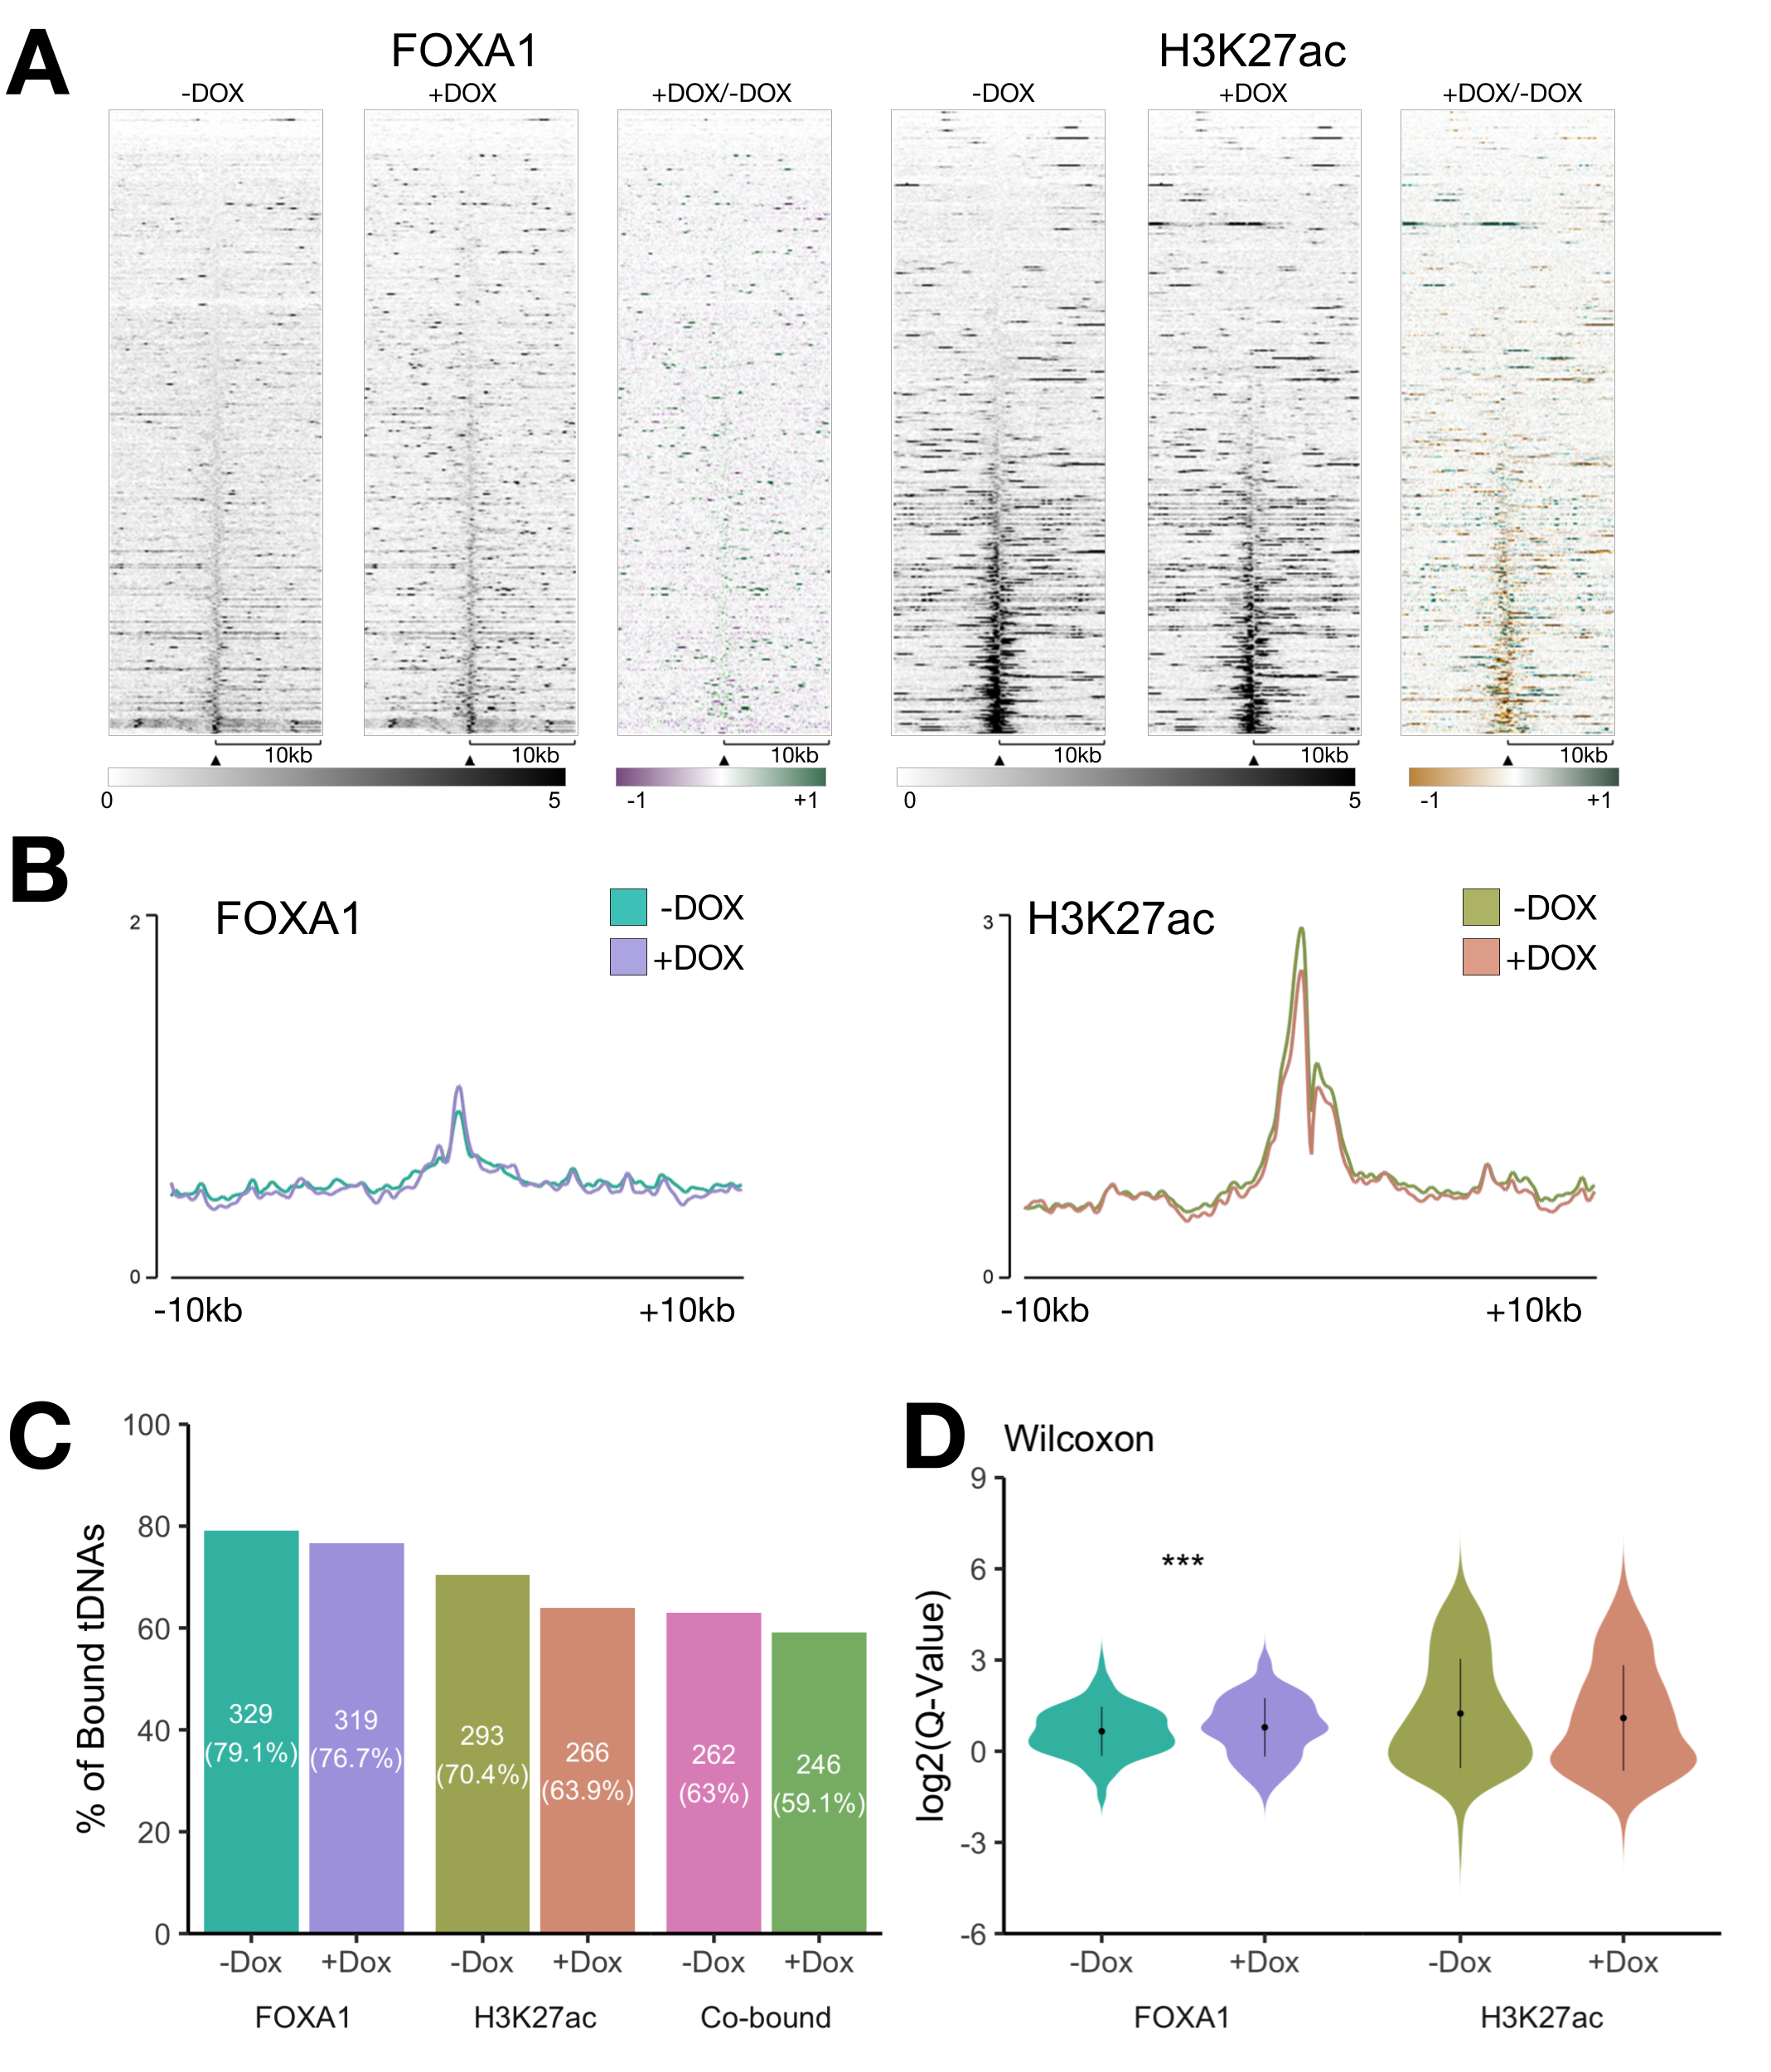
\includegraphics[width=1\linewidth]{../images/results-01} \caption{Comparisons of FOXA1 and H3K27ac binding at tDNAs, with and without Dox.(A) Heatmaps of FOXA1 and H3K27ac across hg19 tRNA genes in MCF-7 cells. Genes arranged in order of increasing -Dox Q-value. Ratiometric heatmaps represent the log2 ratio between -Dox and +Dox peaks. Windows represent ±10kb from the centre of the gene. N = 416. (B) Average signal intensity overlay of FOXA1 and H3K27ac. Windows represent ±10kb from the centre of the gene. (C) Violin plots of FOXA1 and H3K27ac Q-values within ±500bp of the gene body. *p < 0.05.(D) Bar plots of the percentage of cells bound by FOXA1 and H3K27ac. }\label{fig:results-1}
\end{figure}

\hypertarget{foxa1-alters-h3k27ac-binding-levels}{%
\subsection{FOXA1 alters H3K27ac binding levels}\label{foxa1-alters-h3k27ac-binding-levels}}

To elucidate how FOXA1 impacts tDNA levels, tDNAs that were differently enriched upon FOXA1 OE were categorised as gained (UP) and lost (DN) (fold-change \textgreater{} 1.5, \emph{P}-value \textgreater{} 1e-3).
This discovered that substantially more tDNAs gained (UP) FOXA1 binding than lost (DN) (96 vs.~62), whilst 258 tDNAs remained relatively unchanged (Figure \ref{fig:results-2}A, left).
For H3K27ac, 54 tDNAs gained (UP) and 124 lost (DN) H3K27ac (Figure \ref{fig:results-2}A, right), whereas 236 tDNAs remained relatively unchanged.
As expected, Q-values density was significantly increased or decreased at UP and DN tDNAs, respectively (Figure \ref{fig:results-2}B).
For FOXA1, median Q-values decreased 42.7\% at DN tDNAs, and increased 90\% at UP tDNAs.
For H3K27ac, median Q-values decreased 26.4\% at DN tDNAs, and increased 81.5\% at UP tDNAs.

Focusing on UP tDNAs, 95 gain (UP) FOXA1 and 54 gain (UP) H3K27ac (Figure \ref{fig:results-2}C).
Of this subset (n = 150), 14\% gain both FOXA1 and H3K27ac.
Examples of exclusive and co-bound tDNAs are shown in Figure \ref{fig:results-2}D.

SUMMARY

\begin{figure}[H]
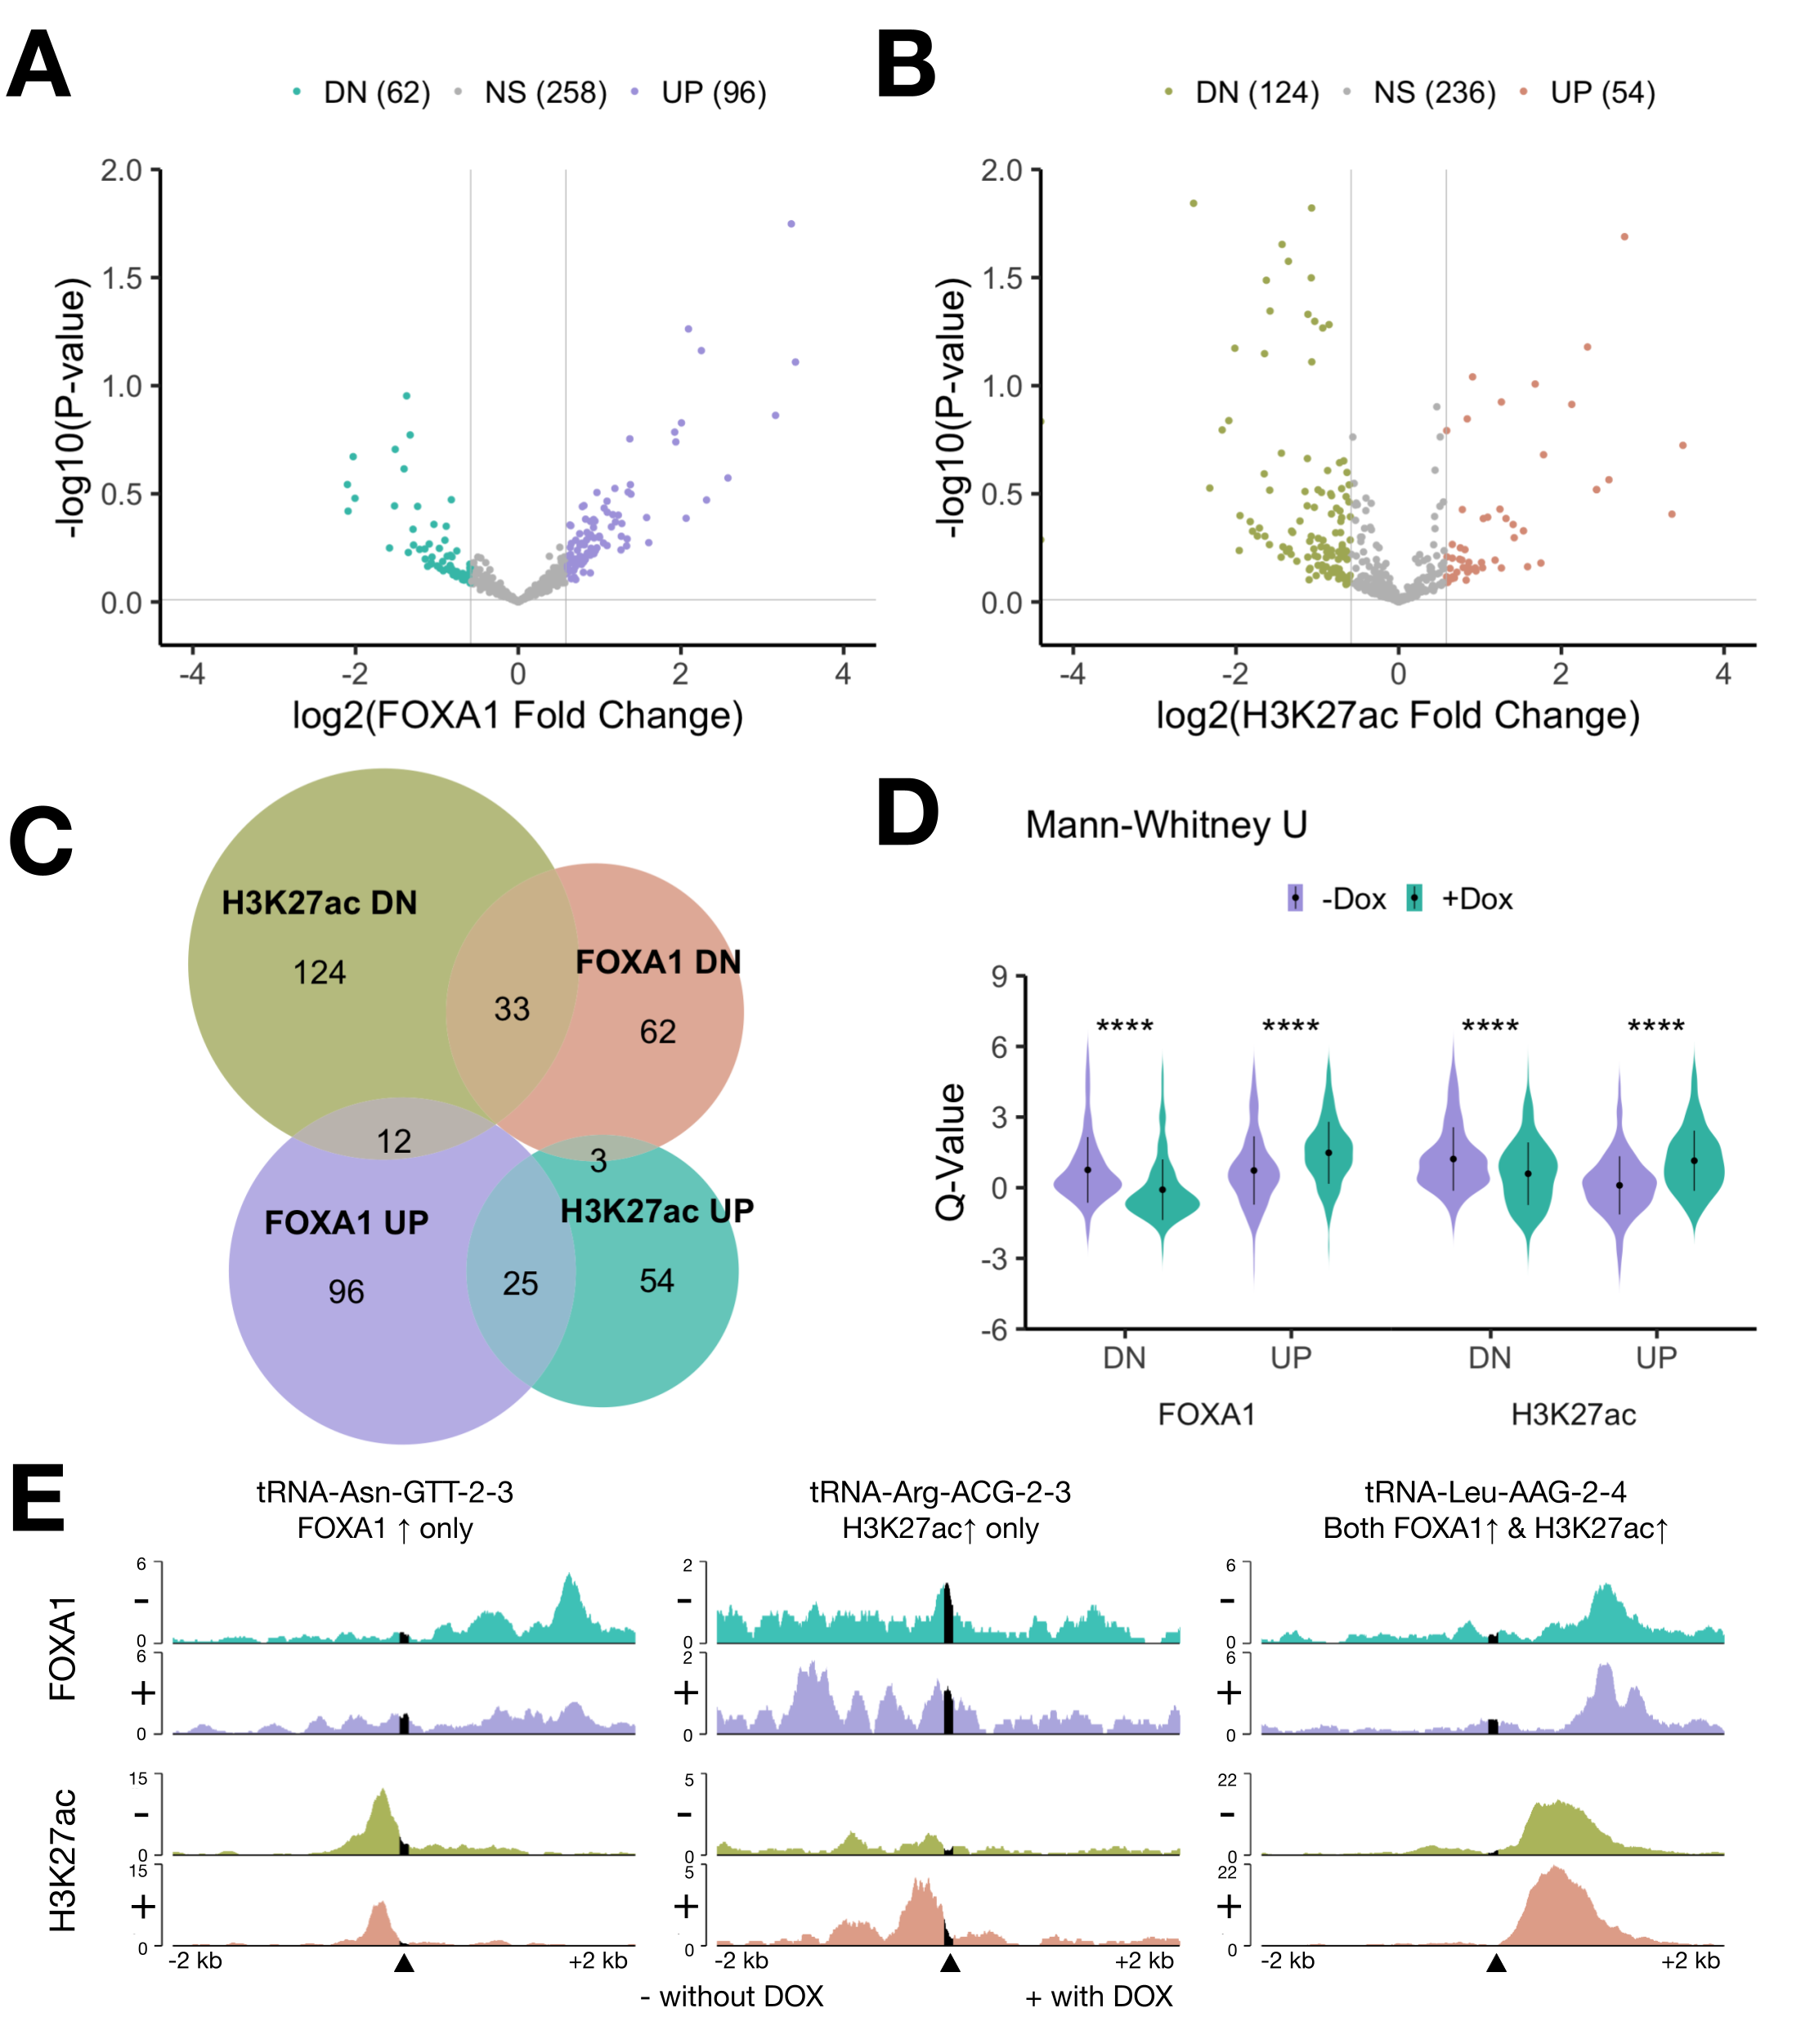
\includegraphics[width=1\linewidth]{../images/results-02} \caption{FOXA1 OE impacts binding of FOXA1 and H3K27ac at tRNA genes. (A) Volcano plots of FOXA1 (n = 416) and H3K27ac (n = 414) Q-values in +Dox vs. −Dox cells. (Left) The purple and green dots correspond to the regions with UP and DN FOXA1, respectively. (Right) The orange and green dots correspond to the regions with UP and DN H3K27ac, respectively. The threhold for calling was set fold-change > 1.5 and P < 1e-3. (B) Violin plots of the Q-values of GAIN or LOSS tRNA genes. ****p < 0.0001. (C) Venn diagram representing the overlap between FOXA1 and H3K27ac GAIN regions. (D) Filltrack examples of seperate and co-occuring FOXA1 and H3K27ac GAIN events within ± 2 kb of tDNAs. The black line represents the gene body.}\label{fig:results-2}
\end{figure}

\hypertarget{tdnas-are-activated-by-foxa1-oe}{%
\subsection{tDNAs are activated by FOXA1 OE}\label{tdnas-are-activated-by-foxa1-oe}}

The next step was to investigate the impact of FOXA1 on tDNA activity.
Almost half of human tDNAs are silent or poorly expressed\textsuperscript{\protect\hyperlink{ref-Torres2019}{59}}.
Thus, tDNAs were classified as `active' if H3K27ac Q-values exceeded the median -DOX value (Q \textgreater{} 1.808).
The Q-value density of inactive tDNAs was somewhat altered (p = 0.043), with median FOXA1 Q-values decreasing 4.9\% (Figure \ref{fig:results-3}A).
The density of active tDNAs did not significantly change, though the median Q-value did decrease 18.9\%.

Overexpression of FOXA1 altered the number of active and inactive tDNAs by just 1 (Supplementary Figures X).
However, 27 tDNAs became inactive (LOSS) and 26 became activate (GAIN), whilst the activity status of 363 (87.3\%) tDNAs remained not changed (NC) (Figure \ref{fig:results-3}B).
As expected, the Q-value density of activated (GAIN) tDNAs was changed upon FOXA1 OE (Figure \ref{fig:results-3}C).
Q-values increased 65.4\% for GAIN tDNAs, decreased 14.2\% for LOSS, decreased 8.3\% for NC tDNAs.
However, these changes were not significant for the last two catagories.

Superimposing GAIN and LOSS tDNAs with UP and DOWN tDNAs (Figure \ref{fig:results-2}C) revealed that, of the 26 tDNAs that become active upon FOXA1 OE, 19 also reasonably gained H3K27ac (H3K27ac UP), and 13 reasonably gain FOXA1 (FOXA1 UP) (Figure \ref{fig:results-3}D).
However, only 9 tDNAs gained both H3K27ac and FOXA1.
Examples of activated tDNAs with increased H3K27ac, FOXA1, or both, are shown in Figure \ref{fig:results-3}E.

SUMMARY

\begin{figure}[H]
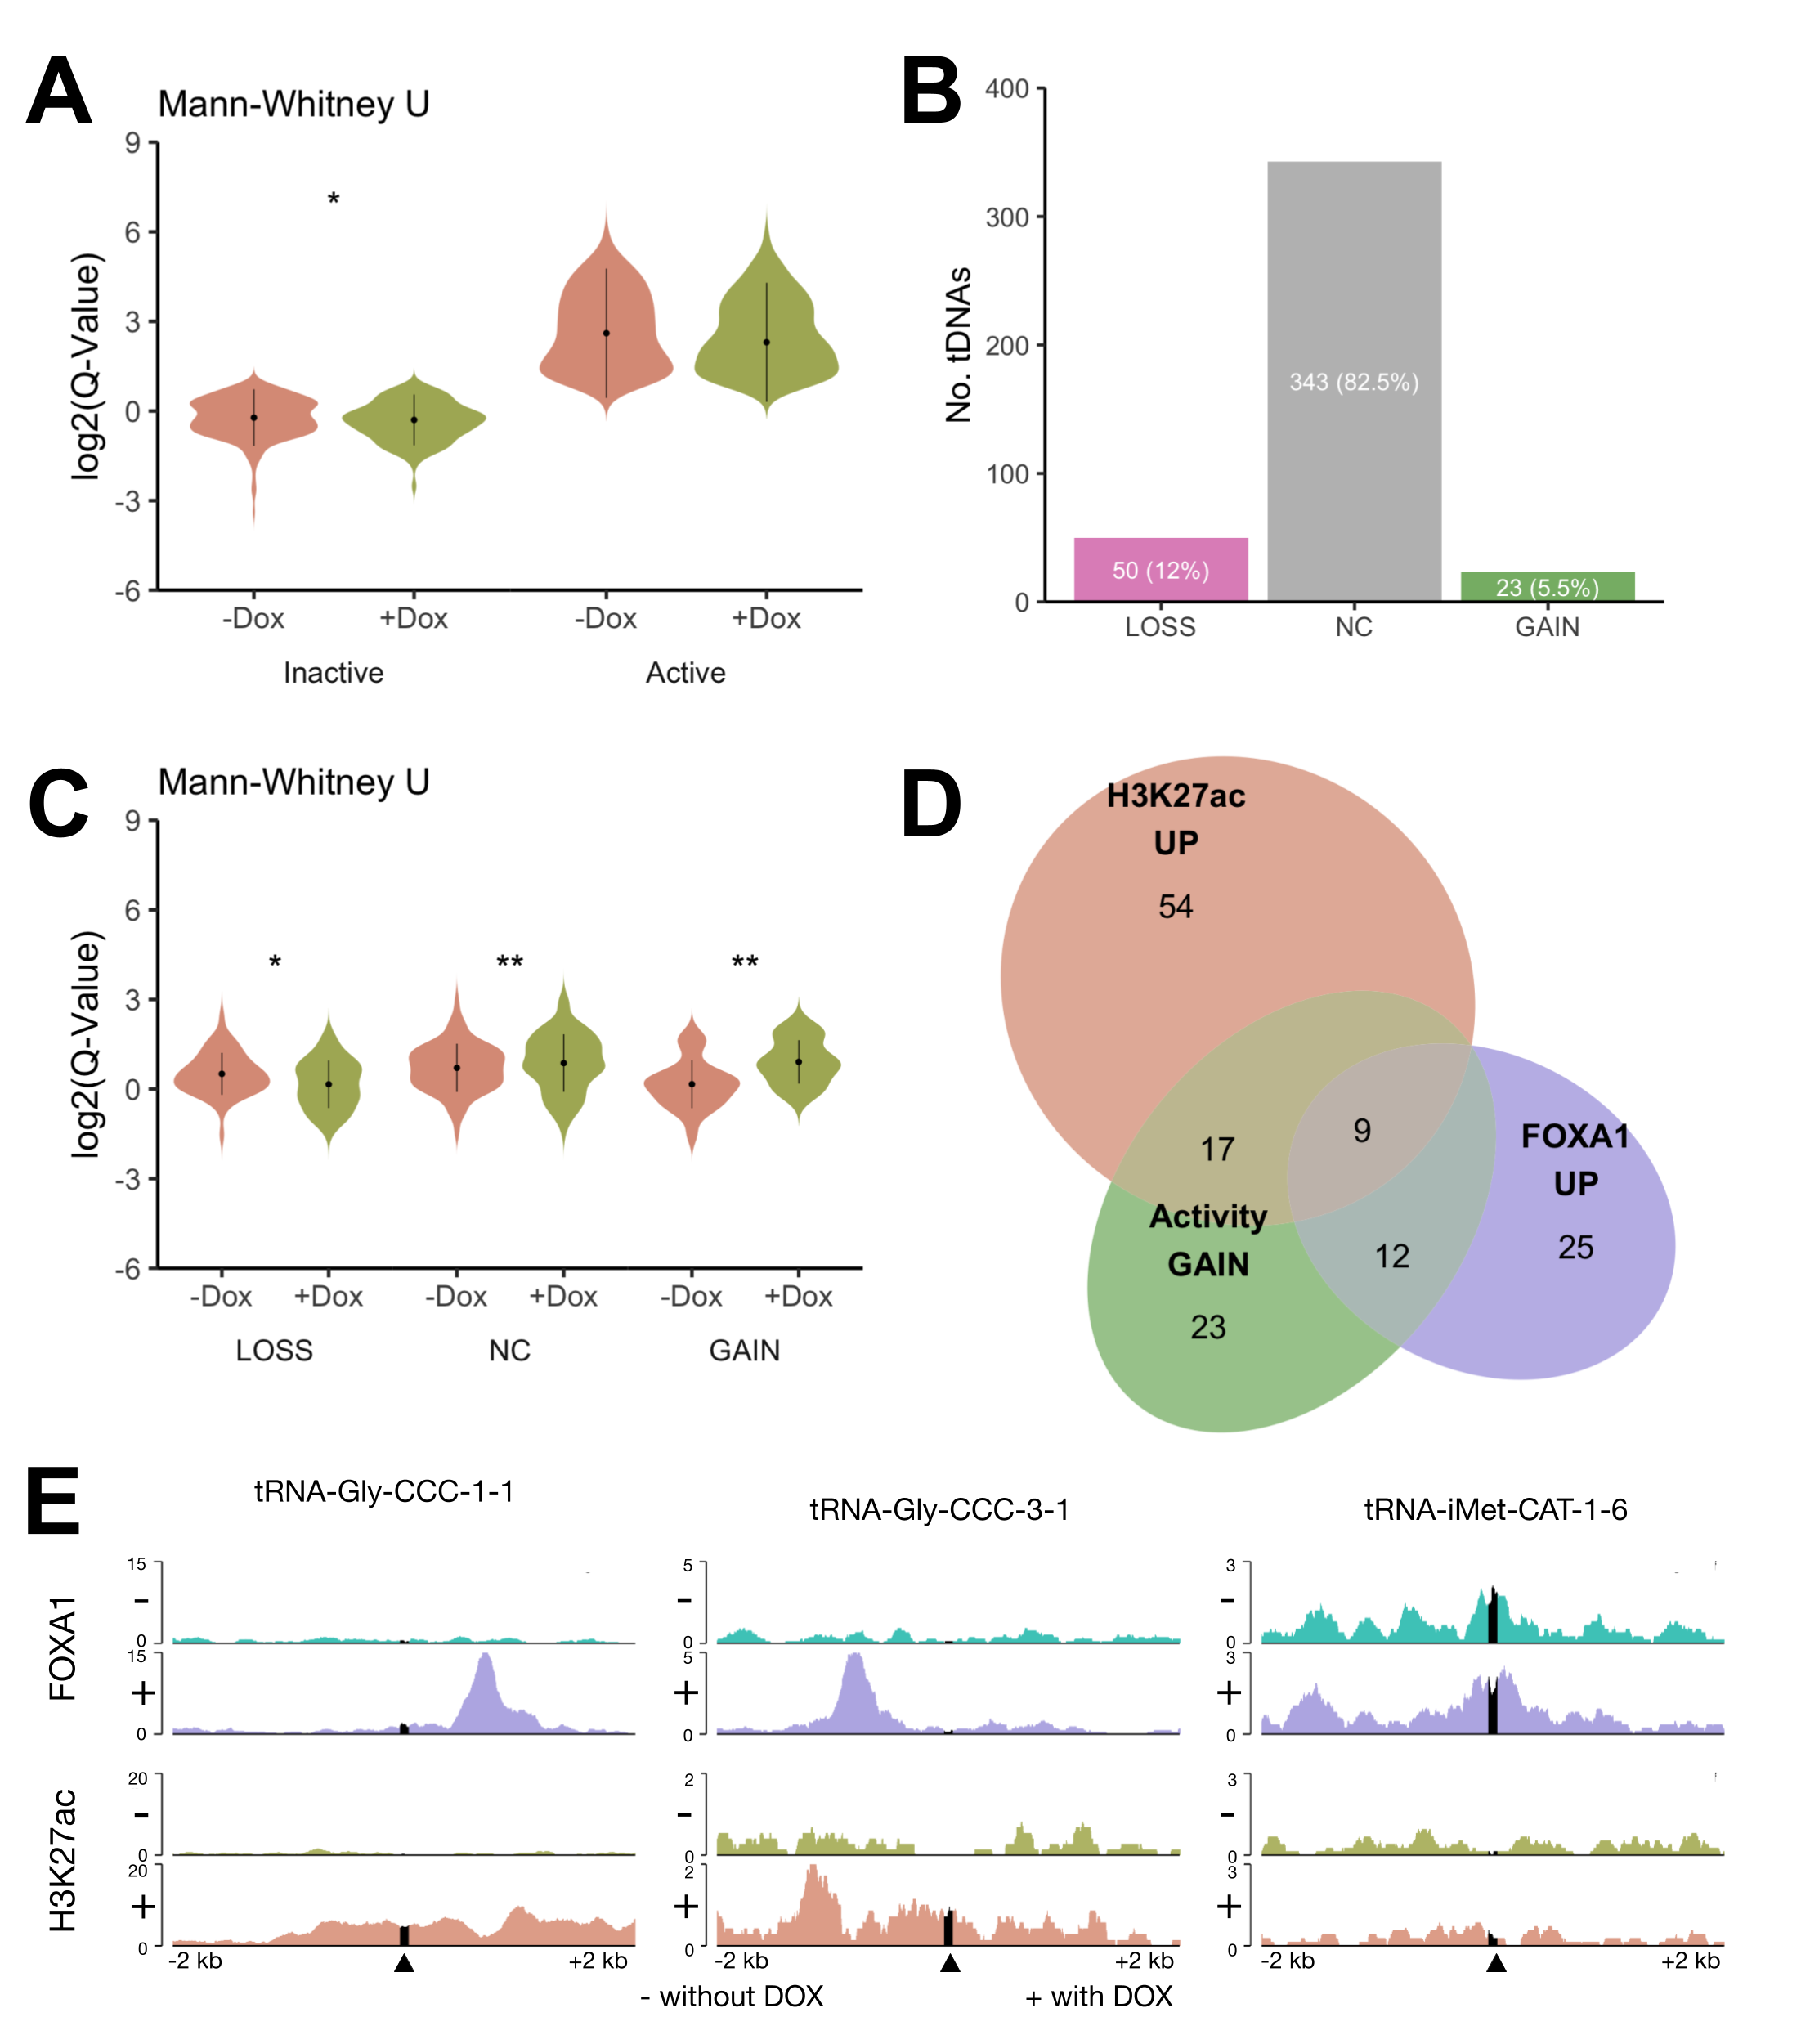
\includegraphics[width=1\linewidth]{../images/results-03} \caption{(A) Violin plot of H3K27ac Q-values within ±500bp of the gene body of inactive and active tDNAs. *p < 0.05. (B) Barplot of tDNAs catagorised by activity change upon FOXA1 OE. tDNAs are classed as inactivated (LOSS), no-change (NC), and activated(GAIN). (C) Violin plot of tDNA Q-values, catagorised as they are in B. *p < 0.05, **p < 0.01. (D) Venn diagram representing the overlap between tDNAs classed as GAIN and UP. (E). Filltrack examples of co-occuring FOXA1 UP and H3K27ac GAIN events within ± 2 kb of tDNAs. The black line represents the gene body.}\label{fig:results-3}
\end{figure}

\hypertarget{foxa1-oe-influences-the-binding-location-of-foxa1-and-h3k27ac}{%
\subsection{FOXA1 OE influences the binding location of FOXA1 and H3K27ac}\label{foxa1-oe-influences-the-binding-location-of-foxa1-and-h3k27ac}}

To assess FOXA1 and H3K27ac binding preference, the levels of FOXA1 and H3K27ac at upstream and downstream regions was quantified within a ± 500 bp (Figure \ref{fig:results-4}A).
The upstream window was classified as the 500 bp region preceding the tDNA loci, including the the TSS.
In contrast, the 500 bp region preceding the TSS defined the downstream region.

FOXA1 was found to be bound at more downstream sites than upstream sites, both with FOXA1 OE and without (-DOX 307 vs 319; +Dox 297 vs 331) (Figure \ref{fig:results-4}B) .
However, FOXA1 did not significantly change the number of FOXA1 bound DNAs upstream or downstream (Figure \ref{fig:results-4}C).
On the other hand, significantly more H3K27ac binding events occured downstream (-DOX 284 vs 280; +Dox 276 vs 240) (Figure \ref{fig:results-4}B).
This pattern of H3K27ac binding was further perpetuated by FOXA1 OE; Q-values significantly decreased 3.8\%\% upstream and 14.3\% downstream (Figure \ref{fig:results-4}C).

\begin{figure}[H]
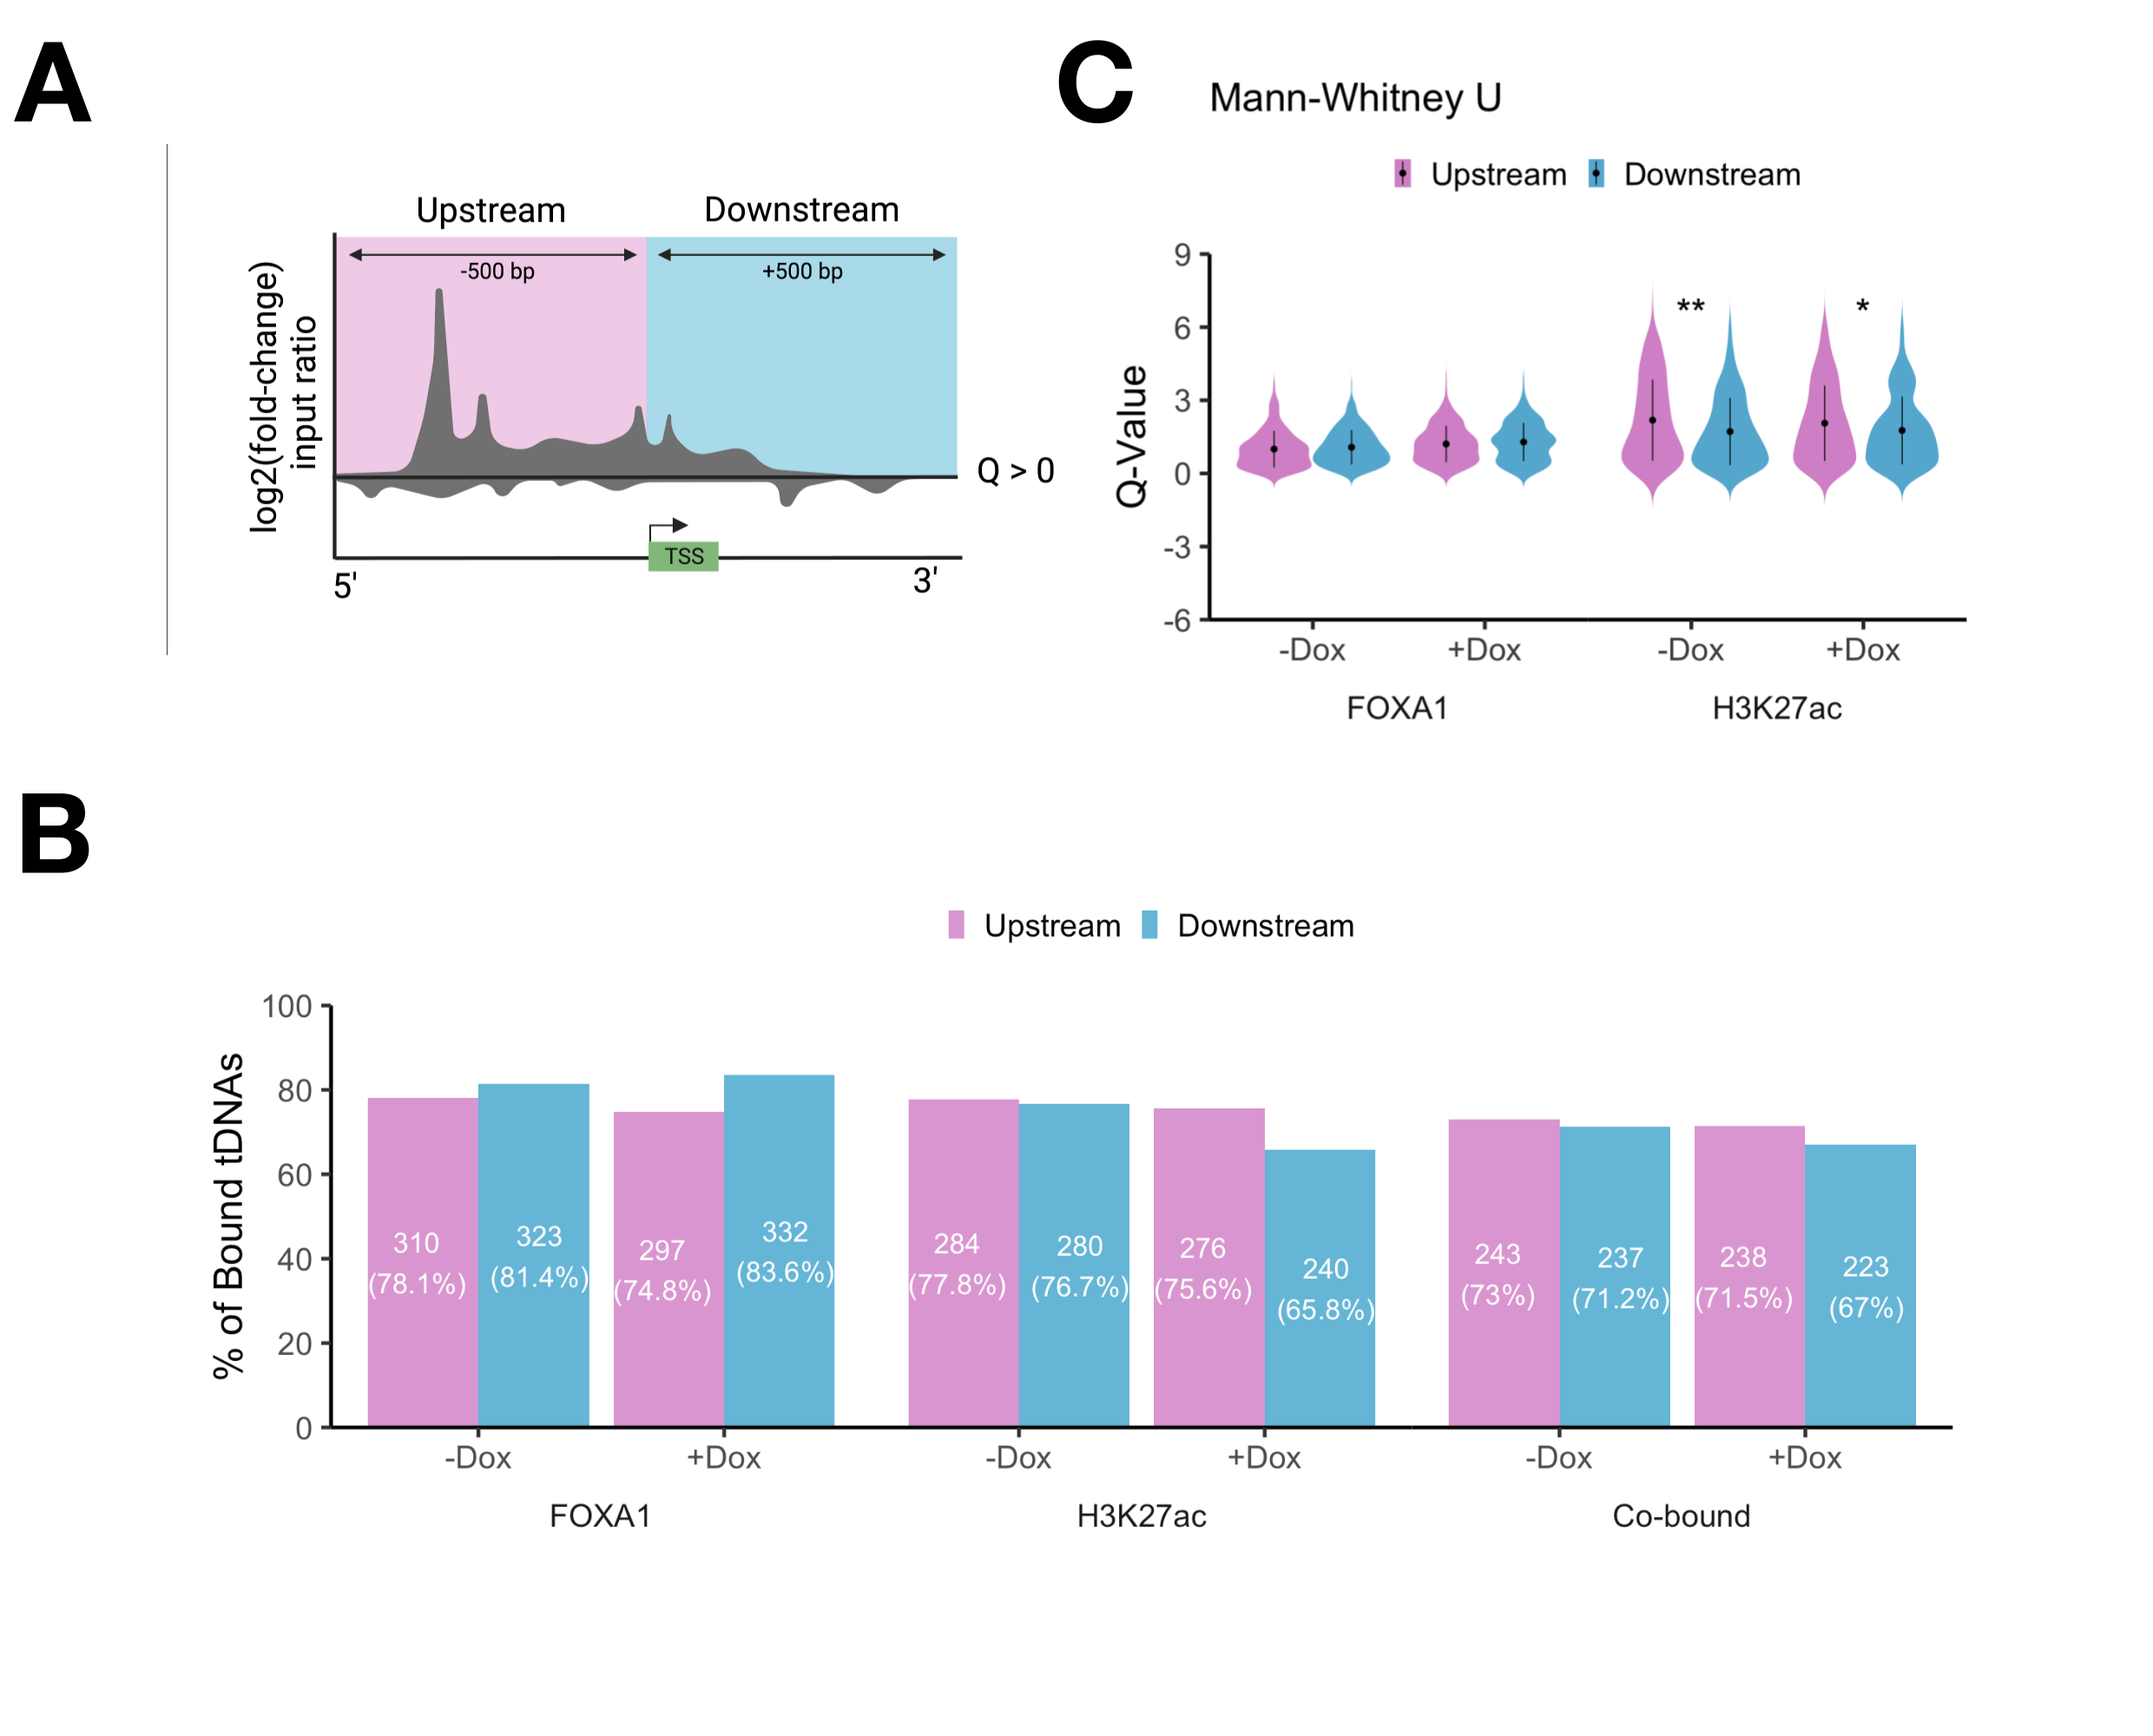
\includegraphics[width=1\linewidth]{../images/results-04} \caption{(A) Schematic of the independent quantification of the upstream and downstream regions of tDNAs. Windows were confined to the ±500 bp, including the gene body. Binding events were counted if Q-values exceeded the input values. (B) Violin plot of the upstream and downstream Q-values for FOXA1 and H3K27ac, with or without Dox. (C)}\label{fig:results-4}
\end{figure}

\hypertarget{motif-analysis-1}{%
\subsection{Motif Analysis}\label{motif-analysis-1}}

\hypertarget{why}{%
\paragraph{Why?}\label{why}}

\hypertarget{what}{%
\subsubsection{What?}\label{what}}

MEME CentriMo to identify de novo motifs that are enriched at tDNAs which gain both FOXA1 and H3k27ac

\begin{itemize}
\item
  relative to other tDNAS (gain/lose, lose/lose, lose/gain)
\item
  FOXA1 not enriched
\item
  Look at ERE, AP-1, others?
\item
  Top 3 motifs (fisher E values) - IRF7, ERR3, NR4A1
\item
  A and B box motifs as a control?
  How?

  \begin{itemize}
  \item
    All downstream
  \item
    tDNAs where `matching sequences' all best matches = code for valine
  \item
    Branched amino acids associated with lower BC risk
  \end{itemize}
\end{itemize}

\hypertarget{suggests}{%
\paragraph{Suggests?}\label{suggests}}

\hypertarget{figure-5}{%
\subsection{Figure 5}\label{figure-5}}

\begin{itemize}
\tightlist
\item
  Localisation of FOXA1 at individual tDNA genes in MCF-7 cells
\end{itemize}

Why?

\begin{itemize}
\item
  tRNAs implicated in cancer
\item
  Are they upregulated?
\item
  Look at gain function/gain h3/fox
\item
  Motif ontology
\item
\end{itemize}

What?

Suggests?

\begin{longtable}[]{@{}ll@{}}
\caption{\label{tab:clusters}.}\tabularnewline
\toprule()
Group & Function \\
\midrule()
\endfirsthead
\toprule()
Group & Function \\
\midrule()
\endhead
ALOXE & Insulator Function\textsuperscript{\protect\hyperlink{ref-raab2011}{27},\protect\hyperlink{ref-sizer2022}{29}} \\
Ebersole & Insulator Function\textsuperscript{\protect\hyperlink{ref-Ebersole2011}{28},\protect\hyperlink{ref-sizer2022}{29}} \\
HES7 & \\
Per1 & \\
TMEM107 & Insulator Function\textsuperscript{\protect\hyperlink{ref-raab2011}{27},\protect\hyperlink{ref-sizer2022}{29}} \\
Arg-CCG & Implicated in Cancer Progression\textsuperscript{\protect\hyperlink{ref-Goodarzi2016}{24}} \\
Glu-TTC & Implicated in Cancer Progression\textsuperscript{\protect\hyperlink{ref-Goodarzi2016}{24}} \\
iMET & Proliferation of Breast Cancer \\
Met & iMet Control \\
SeC & Involved in REDOX\textsuperscript{\protect\hyperlink{ref-Sangha2022}{60}} \\
\bottomrule()
\end{longtable}

\begin{center}\rule{0.5\linewidth}{0.5pt}\end{center}

\hypertarget{discussion}{%
\section{Discussion}\label{discussion}}

\begin{itemize}
\item
  FOXA1 alone not efficient to increase activity

  \begin{itemize}
  \tightlist
  \item
    p300
  \end{itemize}
\item
  FOXA1 moves nucleosomes to make other TF accessible?
\item
  Differences in nucleosome positioning will contribute to the distinct density patterns of modified histones, as nucleosomes are excluded from active tRNA promoters and enriched in flanking regions\textsuperscript{\href{https://www.nature.com/articles/nrg3001\#ref-CR8}{8}}.
\item
  Brf1 required for iMET txn
\item
  Loses fox = weak binding?
\item
  Dynamic vs stable marks
\item
  ATAC-seq
\end{itemize}

\hypertarget{conclusion}{%
\section{Conclusion}\label{conclusion}}

\begin{flushright}
2670 Words
\end{flushright}
\footnotesize

\begin{center}\rule{0.5\linewidth}{0.5pt}\end{center}

\hypertarget{references}{%
\section*{References}\label{references}}
\addcontentsline{toc}{section}{References}

\hypertarget{refs}{}
\begin{CSLReferences}{0}{0}
\leavevmode\vadjust pre{\hypertarget{ref-vannini2012}{}}%
\CSLLeftMargin{1 }%
\CSLRightInline{Vannini A, Cramer P. \href{https://doi.org/10.1016/j.molcel.2012.01.023}{Conservation between the RNA Polymerase I, II, and III Transcription Initiation Machineries}. \emph{Molecular Cell} 2012; \textbf{45}: 439--446.}

\leavevmode\vadjust pre{\hypertarget{ref-dieci2007}{}}%
\CSLLeftMargin{2 }%
\CSLRightInline{Dieci G, Fiorino G, Castelnuovo M, Teichmann M, Pagano A. \href{https://doi.org/10.1016/j.tig.2007.09.001}{The expanding RNA polymerase III transcriptome}. \emph{Trends in Genetics} 2007; \textbf{23}: 614--622.}

\leavevmode\vadjust pre{\hypertarget{ref-Raha2010a}{}}%
\CSLLeftMargin{3 }%
\CSLRightInline{Raha D, Wang Z, Moqtaderi Z, Wu L, Zhong G, Gerstein M \emph{et al.} \href{https://doi.org/10.1073/pnas.0911315106}{Close association of RNA polymerase II and many transcription factors with Pol III genes}. \emph{Proceedings of the National Academy of Sciences} 2010; \textbf{107}: 3639--3644.}

\leavevmode\vadjust pre{\hypertarget{ref-Schramm2002}{}}%
\CSLLeftMargin{4 }%
\CSLRightInline{Schramm L, Hernandez N. \href{https://doi.org/10.1101/gad.1018902}{Recruitment of RNA polymerase III to its target promoters}. \emph{Genes \& Development} 2002; \textbf{16}: 2593--2620.}

\leavevmode\vadjust pre{\hypertarget{ref-Lassar1983}{}}%
\CSLLeftMargin{5 }%
\CSLRightInline{Lassar AB, Martin PL, Roeder RG. \href{https://doi.org/10.1126/science.6356356}{Transcription of Class III Genes: Formation of Preinitiation Complexes}. \emph{Science} 1983; \textbf{222}: 740--748.}

\leavevmode\vadjust pre{\hypertarget{ref-Galli1981}{}}%
\CSLLeftMargin{6 }%
\CSLRightInline{Galli G, Hofstetter H, Birnstiel ML. Two conserved sequence blocks within eukaryotic {tRNA} genes are major promoter elements. \emph{Nature} 1981; \textbf{294}: 626--631.}

\leavevmode\vadjust pre{\hypertarget{ref-schramm2000}{}}%
\CSLLeftMargin{7 }%
\CSLRightInline{Schramm L, Pendergrast PS, Sun Y, Hernandez N. \href{https://doi.org/10.1101/gad.836400}{Different human TFIIIB activities direct RNA polymerase III transcription from TATA-containing and TATA-less promoters}. \emph{Genes \& Development} 2000; \textbf{14}: 2650--2663.}

\leavevmode\vadjust pre{\hypertarget{ref-Khoo1994}{}}%
\CSLLeftMargin{8 }%
\CSLRightInline{Khoo B, Brophy B, Jackson SP. \href{https://doi.org/10.1101/gad.8.23.2879}{Conserved functional domains of the RNA polymerase III general transcription factor BRF.} \emph{Genes \& Development} 1994; \textbf{8}: 2879--2890.}

\leavevmode\vadjust pre{\hypertarget{ref-kassavetis1990}{}}%
\CSLLeftMargin{9 }%
\CSLRightInline{Kassavetis GA, Braun BR, Nguyen LH, Peter Geiduschek E. \href{https://doi.org/10.1016/0092-8674(90)90739-2}{S. cerevisiae TFIIIB is the transcription initiation factor proper of RNA polymerase III, while TFIIIA and TFIIIC are assembly factors}. \emph{Cell} 1990; \textbf{60}: 235--245.}

\leavevmode\vadjust pre{\hypertarget{ref-Brooks1977}{}}%
\CSLLeftMargin{10 }%
\CSLRightInline{Brooks RF. Continuous protein synthesis is required to maintain the probability of entry into {S} phase. \emph{Cell} 1977; \textbf{12}: 311--317.}

\leavevmode\vadjust pre{\hypertarget{ref-Baxter1978}{}}%
\CSLLeftMargin{11 }%
\CSLRightInline{Baxter GC, Stanners CP. The effect of protein degradation on cellular growth characteristics. \emph{Journal of cellular physiology} 1978; \textbf{96}: 139--145.}

\leavevmode\vadjust pre{\hypertarget{ref-Zetterberg1965}{}}%
\CSLLeftMargin{12 }%
\CSLRightInline{Zetterberg A, Killander D. Quantitative cytophotometric and autoradiographic studies on the rate of protein synthesis during interphase in mouse fibroblasts in vitro. \emph{Experimental cell research} 1965; \textbf{40}: 1--11.}

\leavevmode\vadjust pre{\hypertarget{ref-Zhang2018}{}}%
\CSLLeftMargin{13 }%
\CSLRightInline{Zhang Z, Ye Y, Gong J, Ruan H, Liu C-J, Xiang Y \emph{et al.} Global analysis of {tRNA} and translation factor expression reveals a dynamic landscape of translational regulation in human cancers. \emph{Communications biology} 2018; \textbf{1}: 234.}

\leavevmode\vadjust pre{\hypertarget{ref-Pavon-Eternod2009}{}}%
\CSLLeftMargin{14 }%
\CSLRightInline{Pavon-Eternod M, Gomes S, Geslain R, Dai Q, Rosner MR, Pan T. {tRNA} over-expression in breast cancer and functional consequences. \emph{Nucleic acids research} 2009; \textbf{37}: 7268--7280.}

\leavevmode\vadjust pre{\hypertarget{ref-Winter2000}{}}%
\CSLLeftMargin{15 }%
\CSLRightInline{Winter AG, Sourvinos G, Allison SJ, Tosh K, Scott PH, Spandidos DA \emph{et al.} {RNA} polymerase {III} transcription factor {TFIIIC2} is overexpressed in ovarian tumors. \emph{Proceedings of the National Academy of Sciences of the United States of America} 2000; \textbf{97}: 12619--12624.}

\leavevmode\vadjust pre{\hypertarget{ref-Krishnan2016}{}}%
\CSLLeftMargin{16 }%
\CSLRightInline{Krishnan P, Ghosh S, Wang B, Heyns M, Li D, Mackey JR \emph{et al.} Genome-wide profiling of transfer {RNAs} and their role as novel prognostic markers for breast cancer. \emph{Scientific reports} 2016; \textbf{6}: 32843.}

\leavevmode\vadjust pre{\hypertarget{ref-White1996}{}}%
\CSLLeftMargin{17 }%
\CSLRightInline{White RJ, Trouche D, Martin K, Jackson SP, Kouzarides T. Repression of {RNA} polymerase {III} transcription by the retinoblastoma protein. \emph{Nature} 1996; \textbf{382}: 88--90.}

\leavevmode\vadjust pre{\hypertarget{ref-Cairns1998}{}}%
\CSLLeftMargin{18 }%
\CSLRightInline{Cairns CA, White RJ. p53 is a general repressor of {RNA} polymerase {III} transcription. \emph{The EMBO journal} 1998; \textbf{17}: 3112--3123.}

\leavevmode\vadjust pre{\hypertarget{ref-Sutcliffe2000}{}}%
\CSLLeftMargin{19 }%
\CSLRightInline{Sutcliffe JE, Brown TR, Allison SJ, Scott PH, White RJ. Retinoblastoma protein disrupts interactions required for {RNA} polymerase {III} transcription. \emph{Molecular and cellular biology} 2000; \textbf{20}: 9192--9202.}

\leavevmode\vadjust pre{\hypertarget{ref-Crighton2003}{}}%
\CSLLeftMargin{20 }%
\CSLRightInline{Crighton D, Woiwode A, Zhang C, Mandavia N, Morton JP, Warnock LJ \emph{et al.} p53 represses {RNA} polymerase {III} transcription by targeting {TBP} and inhibiting promoter occupancy by {TFIIIB}. \emph{The EMBO journal} 2003; \textbf{22}: 2810--2820.}

\leavevmode\vadjust pre{\hypertarget{ref-Gomez-Roman2003}{}}%
\CSLLeftMargin{21 }%
\CSLRightInline{Gomez-Roman N, Grandori C, Eisenman RN, White RJ. Direct activation of {RNA} polymerase {III} transcription by c-myc. \emph{Nature} 2003; \textbf{421}: 290--294.}

\leavevmode\vadjust pre{\hypertarget{ref-Felton-Edkins2003}{}}%
\CSLLeftMargin{22 }%
\CSLRightInline{Felton-Edkins ZA, Fairley JA, Graham EL, Johnston IM, White RJ, Scott PH. The mitogen-activated protein ({MAP}) kinase {ERK} induces {tRNA} synthesis by phosphorylating {TFIIIB}. \emph{The EMBO journal} 2003; \textbf{22}: 2422--2432.}

\leavevmode\vadjust pre{\hypertarget{ref-kuchino1978}{}}%
\CSLLeftMargin{23 }%
\CSLRightInline{Kuchino Y, Borek E. \href{https://doi.org/10.1038/271126a0}{Tumour-specific phenylalanine tRNA contains two supernumerary methylated bases}. \emph{Nature} 1978; \textbf{271}: 126--129.}

\leavevmode\vadjust pre{\hypertarget{ref-Goodarzi2016}{}}%
\CSLLeftMargin{24 }%
\CSLRightInline{Goodarzi H, Nguyen HCB, Zhang S, Dill BD, Molina H, Tavazoie SF. \href{https://doi.org/10.1016/j.cell.2016.05.046}{Modulated Expression of Specific tRNAs Drives Gene Expression and Cancer Progression}. \emph{Cell} 2016; \textbf{165}: 1416--1427.}

\leavevmode\vadjust pre{\hypertarget{ref-Pavon-Eternod2013}{}}%
\CSLLeftMargin{25 }%
\CSLRightInline{Pavon-Eternod M, Gomes S, Rosner MR, Pan T. \href{https://doi.org/10.1261/rna.037507.112}{Overexpression of initiator methionine tRNA leads to global reprogramming of tRNA expression and increased proliferation in human epithelial cells}. \emph{RNA} 2013; \textbf{19}: 461--466.}

\leavevmode\vadjust pre{\hypertarget{ref-Birch2016}{}}%
\CSLLeftMargin{26 }%
\CSLRightInline{Birch J, Clarke CJ, Campbell AD, Campbell K, Mitchell L, Liko D \emph{et al.} The initiator methionine {tRNA} drives cell migration and invasion leading to increased metastatic potential in melanoma. \emph{Biology open} 2016; \textbf{5}: 1371--1379.}

\leavevmode\vadjust pre{\hypertarget{ref-raab2011}{}}%
\CSLLeftMargin{27 }%
\CSLRightInline{Raab JR, Chiu J, Zhu J, Katzman S, Kurukuti S, Wade PA \emph{et al.} \href{https://doi.org/10.1038/emboj.2011.406}{Human tRNA genes function as chromatin insulators}. \emph{The EMBO Journal} 2011; \textbf{31}: 330--350.}

\leavevmode\vadjust pre{\hypertarget{ref-Ebersole2011}{}}%
\CSLLeftMargin{28 }%
\CSLRightInline{Ebersole T, Kim J-H, Samoshkin A, Kouprina N, Pavlicek A, White RJ \emph{et al.} \href{https://doi.org/10.4161/cc.10.16.17092}{tRNA genes protect a reporter gene from epigenetic silencing in mouse cells}. \emph{Cell Cycle} 2011; \textbf{10}: 2779--2791.}

\leavevmode\vadjust pre{\hypertarget{ref-sizer2022}{}}%
\CSLLeftMargin{29 }%
\CSLRightInline{Sizer RE, Chahid N, Butterfield SP, Donze D, Bryant NJ, White RJ. \href{https://doi.org/10.1016/j.gene.2022.146533}{TFIIIC-based chromatin insulators through eukaryotic evolution}. \emph{Gene} 2022; \textbf{835}: 146533.}

\leavevmode\vadjust pre{\hypertarget{ref-Sung2021}{}}%
\CSLLeftMargin{30 }%
\CSLRightInline{Sung H, Ferlay J, Siegel RL, Laversanne M, Soerjomataram I, Jemal A \emph{et al.} Global cancer statistics 2020: {GLOBOCAN} estimates of incidence and mortality worldwide for 36 cancers in 185 countries. \emph{CA: a cancer journal for clinicians} 2021; \textbf{71}: 209--249.}

\leavevmode\vadjust pre{\hypertarget{ref-allred2004}{}}%
\CSLLeftMargin{31 }%
\CSLRightInline{Allred DC, Brown P, Medina D. The origins of estrogen receptor alpha-positive and estrogen receptor alpha-negative human breast cancer. \emph{Breast Cancer Research} 2004; \textbf{6}. doi:\href{https://doi.org/10.1186/bcr938}{10.1186/bcr938}.}

\leavevmode\vadjust pre{\hypertarget{ref-Johnston2018}{}}%
\CSLLeftMargin{32 }%
\CSLRightInline{Johnston SJ, Cheung K-L. Endocrine therapy for breast cancer: A model of hormonal manipulation. \emph{Oncology and therapy} 2018; \textbf{6}: 141--156.}

\leavevmode\vadjust pre{\hypertarget{ref-Anurag2018}{}}%
\CSLLeftMargin{33 }%
\CSLRightInline{Anurag M, Ellis MJ, Haricharan S. {DNA} damage repair defects as a new class of endocrine treatment resistance driver. \emph{Oncotarget} 2018; \textbf{9}: 36252--36253.}

\leavevmode\vadjust pre{\hypertarget{ref-Costa1989}{}}%
\CSLLeftMargin{34 }%
\CSLRightInline{Costa RH, Grayson DR, Darnell JE Jr. Multiple hepatocyte-enriched nuclear factors function in the regulation of transthyretin and alpha 1-antitrypsin genes. \emph{Molecular and cellular biology} 1989; \textbf{9}: 1415--1425.}

\leavevmode\vadjust pre{\hypertarget{ref-Cirillo2002}{}}%
\CSLLeftMargin{35 }%
\CSLRightInline{Cirillo LA, Lin FR, Cuesta I, Friedman D, Jarnik M, Zaret KS. Opening of compacted chromatin by early developmental transcription factors {HNF3} ({FoxA}) and {GATA-4}. \emph{Molecular cell} 2002; \textbf{9}: 279--289.}

\leavevmode\vadjust pre{\hypertarget{ref-carroll2005}{}}%
\CSLLeftMargin{36 }%
\CSLRightInline{Carroll JS, Liu XS, Brodsky AS, Li W, Meyer CA, Szary AJ \emph{et al.} \href{https://doi.org/10.1016/j.cell.2005.05.008}{Chromosome-Wide Mapping of Estrogen Receptor Binding Reveals Long-Range Regulation Requiring the Forkhead Protein FoxA1}. \emph{Cell} 2005; \textbf{122}: 33--43.}

\leavevmode\vadjust pre{\hypertarget{ref-laganiuxe8re2005}{}}%
\CSLLeftMargin{37 }%
\CSLRightInline{Laganière J, Deblois G, Lefebvre C, Bataille AR, Robert F, Giguère V. \href{https://doi.org/10.1073/pnas.0505575102}{Location analysis of estrogen receptor α target promoters reveals that FOXA1 defines a domain of the estrogen response}. \emph{Proceedings of the National Academy of Sciences} 2005; \textbf{102}: 11651--11656.}

\leavevmode\vadjust pre{\hypertarget{ref-Hurtado2011}{}}%
\CSLLeftMargin{38 }%
\CSLRightInline{Hurtado A, Holmes KA, Ross-Innes CS, Schmidt D, Carroll JS. FOXA1 is a key determinant of estrogen receptor function and endocrine response. \emph{Apollo - University of Cambridge Repository} 2021. doi:\href{https://doi.org/10.17863/CAM.63405}{10.17863/CAM.63405}.}

\leavevmode\vadjust pre{\hypertarget{ref-Wolf2007}{}}%
\CSLLeftMargin{39 }%
\CSLRightInline{Wolf I, Bose S, Williamson EA, Miller CW, Karlan BY, Koeffler HP. {FOXA1}: Growth inhibitor and a favorable prognostic factor in human breast cancer. \emph{International journal of cancer Journal international du cancer} 2007; \textbf{120}: 1013--1022.}

\leavevmode\vadjust pre{\hypertarget{ref-Williamson2006}{}}%
\CSLLeftMargin{40 }%
\CSLRightInline{Williamson EA, Wolf I, O'Kelly J, Bose S, Tanosaki S, Koeffler HP. {BRCA1} and {FOXA1} proteins coregulate the expression of the cell cycle-dependent kinase inhibitor p27(Kip1). \emph{Oncogene} 2006; \textbf{25}: 1391--1399.}

\leavevmode\vadjust pre{\hypertarget{ref-Tsuchiya1999}{}}%
\CSLLeftMargin{41 }%
\CSLRightInline{Tsuchiya A, Zhang GJ, Kanno M. Prognostic impact of cyclin-dependent kinase inhibitor p27kip1 in node-positive breast cancer. \emph{Journal of surgical oncology} 1999; \textbf{70}: 230--234.}

\leavevmode\vadjust pre{\hypertarget{ref-Fredersdorf1997}{}}%
\CSLLeftMargin{42 }%
\CSLRightInline{Fredersdorf S, Burns J, Milne AM, Packham G, Fallis L, Gillett CE \emph{et al.} High level expression of p27\(^{kip1}\) and cyclin {D1} in some human breast cancer cells: Inverse correlation between the expression of p27\(^{kip1}\) and degree of malignancy in human breast and colorectal cancers. \emph{Proceedings of the National Academy of Sciences} 1997; \textbf{94}: 6380--6385.}

\leavevmode\vadjust pre{\hypertarget{ref-Badve2007}{}}%
\CSLLeftMargin{43 }%
\CSLRightInline{Badve S, Turbin D, Thorat MA, Morimiya A, Nielsen TO, Perou CM \emph{et al.} {FOXA1} expression in breast cancer--correlation with luminal subtype a and survival. \emph{Clinical cancer research: an official journal of the American Association for Cancer Research} 2007; \textbf{13}: 4415--4421.}

\leavevmode\vadjust pre{\hypertarget{ref-ross-innes2012}{}}%
\CSLLeftMargin{44 }%
\CSLRightInline{Ross-Innes CS, Stark R, Teschendorff AE, Holmes KA, Ali HR, Dunning MJ \emph{et al.} \href{https://doi.org/10.1038/nature10730}{Differential oestrogen receptor binding is associated with clinical outcome in breast cancer}. \emph{Nature} 2012; \textbf{481}: 389--393.}

\leavevmode\vadjust pre{\hypertarget{ref-Fu2016}{}}%
\CSLLeftMargin{45 }%
\CSLRightInline{Fu X, Jeselsohn R, Pereira R, Hollingsworth EF, Creighton CJ, Li F \emph{et al.} {FOXA1} overexpression mediates endocrine resistance by altering the {ER} transcriptome and {IL-8} expression in {ER-positive} breast cancer. \emph{Proceedings of the National Academy of Sciences of the United States of America} 2016; \textbf{113}: E6600--E6609.}

\leavevmode\vadjust pre{\hypertarget{ref-Hah2011}{}}%
\CSLLeftMargin{46 }%
\CSLRightInline{Hah N, Danko CG, Core L, Waterfall JJ, Siepel A, Lis JT \emph{et al.} A rapid, extensive, and transient transcriptional response to estrogen signaling in breast cancer cells. \emph{Cell} 2011; \textbf{145}: 622--634.}

\leavevmode\vadjust pre{\hypertarget{ref-zhong2014}{}}%
\CSLLeftMargin{47 }%
\CSLRightInline{Zhong Q, Shi G, Zhang Q, Lu L, Levy D, Zhong S. \href{https://doi.org/10.18632/oncotarget.2678}{Tamoxifen represses alcohol-induced transcription of RNA polymerase III-dependent genes in breast cancer cells}. \emph{Oncotarget} 2014; \textbf{5}: 12410--12417.}

\leavevmode\vadjust pre{\hypertarget{ref-fu2019}{}}%
\CSLLeftMargin{48 }%
\CSLRightInline{Fu X, Pereira R, De Angelis C, Veeraraghavan J, Nanda S, Qin L \emph{et al.} \href{https://doi.org/10.1073/pnas.1911584116}{FOXA1 upregulation promotes enhancer and transcriptional reprogramming in endocrine-resistant breast cancer}. \emph{Proceedings of the National Academy of Sciences} 2019; \textbf{116}: 26823--26834.}

\leavevmode\vadjust pre{\hypertarget{ref-leinonen2010}{}}%
\CSLLeftMargin{49 }%
\CSLRightInline{Leinonen R, Sugawara H, Shumway M. \href{https://doi.org/10.1093/nar/gkq1019}{The Sequence Read Archive}. \emph{Nucleic Acids Research} 2010; \textbf{39}: D19--D21.}

\leavevmode\vadjust pre{\hypertarget{ref-thegala2022}{}}%
\CSLLeftMargin{50 }%
\CSLRightInline{Afgan E, Nekrutenko A, Grüning BA, Blankenberg D, Goecks J, Schatz MC \emph{et al.} \href{https://doi.org/10.1093/nar/gkac247}{The Galaxy platform for accessible, reproducible and collaborative biomedical analyses: 2022 update}. \emph{Nucleic Acids Research} 2022; \textbf{50}: W345--W351.}

\leavevmode\vadjust pre{\hypertarget{ref-langmead2012}{}}%
\CSLLeftMargin{51 }%
\CSLRightInline{Langmead B, Salzberg SL. \href{https://doi.org/10.1038/nmeth.1923}{Fast gapped-read alignment with Bowtie 2}. \emph{Nature Methods} 2012; \textbf{9}: 357--359.}

\leavevmode\vadjust pre{\hypertarget{ref-Karolchik2004}{}}%
\CSLLeftMargin{52 }%
\CSLRightInline{Karolchik D. \href{https://doi.org/10.1093/nar/gkh103}{The UCSC Table Browser data retrieval tool}. \emph{Nucleic Acids Research} 2004; \textbf{32}: 493D--496.}

\leavevmode\vadjust pre{\hypertarget{ref-Chan2016}{}}%
\CSLLeftMargin{53 }%
\CSLRightInline{Chan PP, Lowe TM. \href{https://doi.org/10.1093/nar/gkv1309}{GtRNAdb 2.0: an expanded database of transfer RNA genes identified in complete and draft genomes}. \emph{Nucleic Acids Research} 2015; \textbf{44}: D184--D189.}

\leavevmode\vadjust pre{\hypertarget{ref-lerdrup2016}{}}%
\CSLLeftMargin{54 }%
\CSLRightInline{Lerdrup M, Johansen JV, Agrawal-Singh S, Hansen K. \href{https://doi.org/10.1038/nsmb.3180}{An interactive environment for agile analysis and visualization of ChIP-sequencing data}. \emph{Nature Structural \& Molecular Biology} 2016; \textbf{23}: 349--357.}

\leavevmode\vadjust pre{\hypertarget{ref-r}{}}%
\CSLLeftMargin{55 }%
\CSLRightInline{R Core Team. \emph{R: A language and environment for statistical computing}. R Foundation for Statistical Computing: Vienna, Austria, 2023. \url{https://www.R-project.org/}.}

\leavevmode\vadjust pre{\hypertarget{ref-wickham2019}{}}%
\CSLLeftMargin{56 }%
\CSLRightInline{Wickham H, Averick M, Bryan J, Chang W, McGowan L, François R \emph{et al.} \href{https://doi.org/10.21105/joss.01686}{Welcome to the tidyverse}. \emph{Journal of Open Source Software} 2019; \textbf{4}: 1686.}

\leavevmode\vadjust pre{\hypertarget{ref-ggpubr}{}}%
\CSLLeftMargin{57 }%
\CSLRightInline{Kassambara A. \emph{Ggpubr: 'ggplot2' based publication ready plots}. 2023\url{https://CRAN.R-project.org/package=ggpubr}.}

\leavevmode\vadjust pre{\hypertarget{ref-fu2016}{}}%
\CSLLeftMargin{58 }%
\CSLRightInline{Fu X, Jeselsohn R, Pereira R, Hollingsworth EF, Creighton CJ, Li F \emph{et al.} FOXA1 overexpression mediates endocrine resistance by altering the ER transcriptome and IL-8 expression in ER-positive breast cancer. \emph{Proceedings of the National Academy of Sciences} 2016; \textbf{113}. doi:\href{https://doi.org/10.1073/pnas.1612835113}{10.1073/pnas.1612835113}.}

\leavevmode\vadjust pre{\hypertarget{ref-Torres2019}{}}%
\CSLLeftMargin{59 }%
\CSLRightInline{Torres AG. \href{https://doi.org/10.1177/1177932219868454}{Enjoy the Silence: Nearly Half of Human tRNA Genes Are Silent}. \emph{Bioinformatics and Biology Insights} 2019; \textbf{13}: 117793221986845.}

\leavevmode\vadjust pre{\hypertarget{ref-Sangha2022}{}}%
\CSLLeftMargin{60 }%
\CSLRightInline{Sangha AK, Kantidakis T. \href{https://doi.org/10.3390/cimb44070207}{The Aminoacyl-tRNA Synthetase and tRNA Expression Levels Are Deregulated in Cancer and Correlate Independently with Patient Survival}. \emph{Current Issues in Molecular Biology} 2022; \textbf{44}: 3001--3019.}

\end{CSLReferences}

\end{document}
